%versi 3 (22-07-2020)
\chapter{Landasan Teori}
\label{chap:landasan_teori}

\section{Point of Interest}
\label{sec:poi}

\textit{Point of Interest} (POI) adalah sebuah lokasi geografis yang memiliki kegunaan tertentu. POI biasanya dikenali oleh banyak orang dan memiliki keunikan tertentu pada tampilannya. Salah satu contoh POI dapat dilihat pada Gambar~\ref{fig:poi}. POI juga dapat dimanfaatkan untuk menjadi penanda lokasi seseorang. Seseorang dapat mengerti lokasinya dengan melihat POI yang ada di sekitarnya.
\begin{figure}[H]
	\centering
	\includegraphics[width=0.6\linewidth]{poi.png}
	\caption{Salah satu contoh POI.}
	\label{fig:poi}
\end{figure}

Beberapa POI tertentu dapat memiliki logo yang sifatnya unik. POI tersebut dapat dikenali dengan hanya melihat logonya saja. Contoh bisa dilihat pada Gambar~\ref{fig:poi_logo}. POI dengan logo unik ini dapat dikenali oleh komputer salah satunya dengan menggunakan teknik \textit{Object Instance Recognition} (OIR). 
\begin{figure}[H]
	\centering
	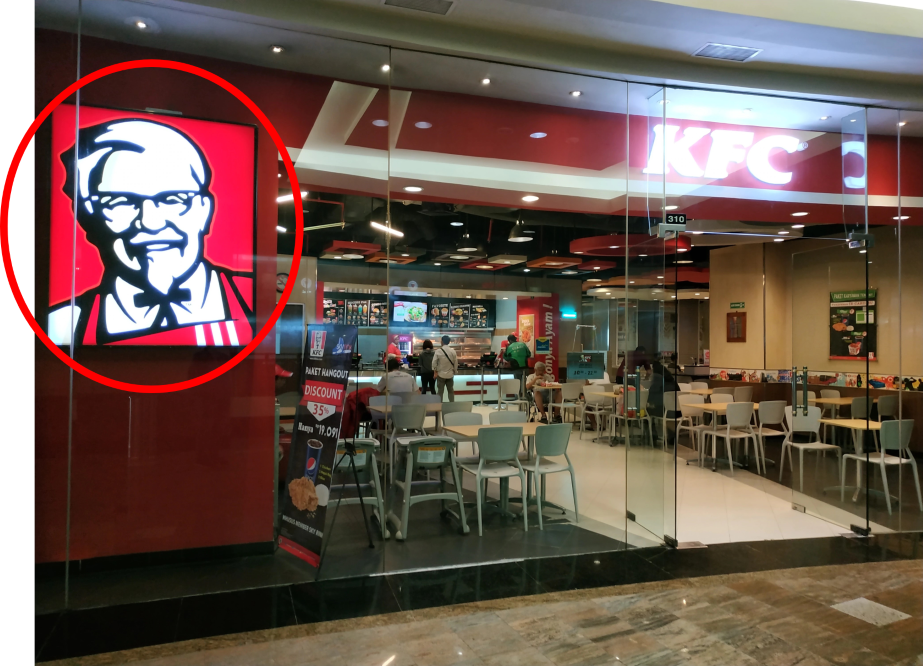
\includegraphics[width=0.35\linewidth]{kfc_circled.png}
	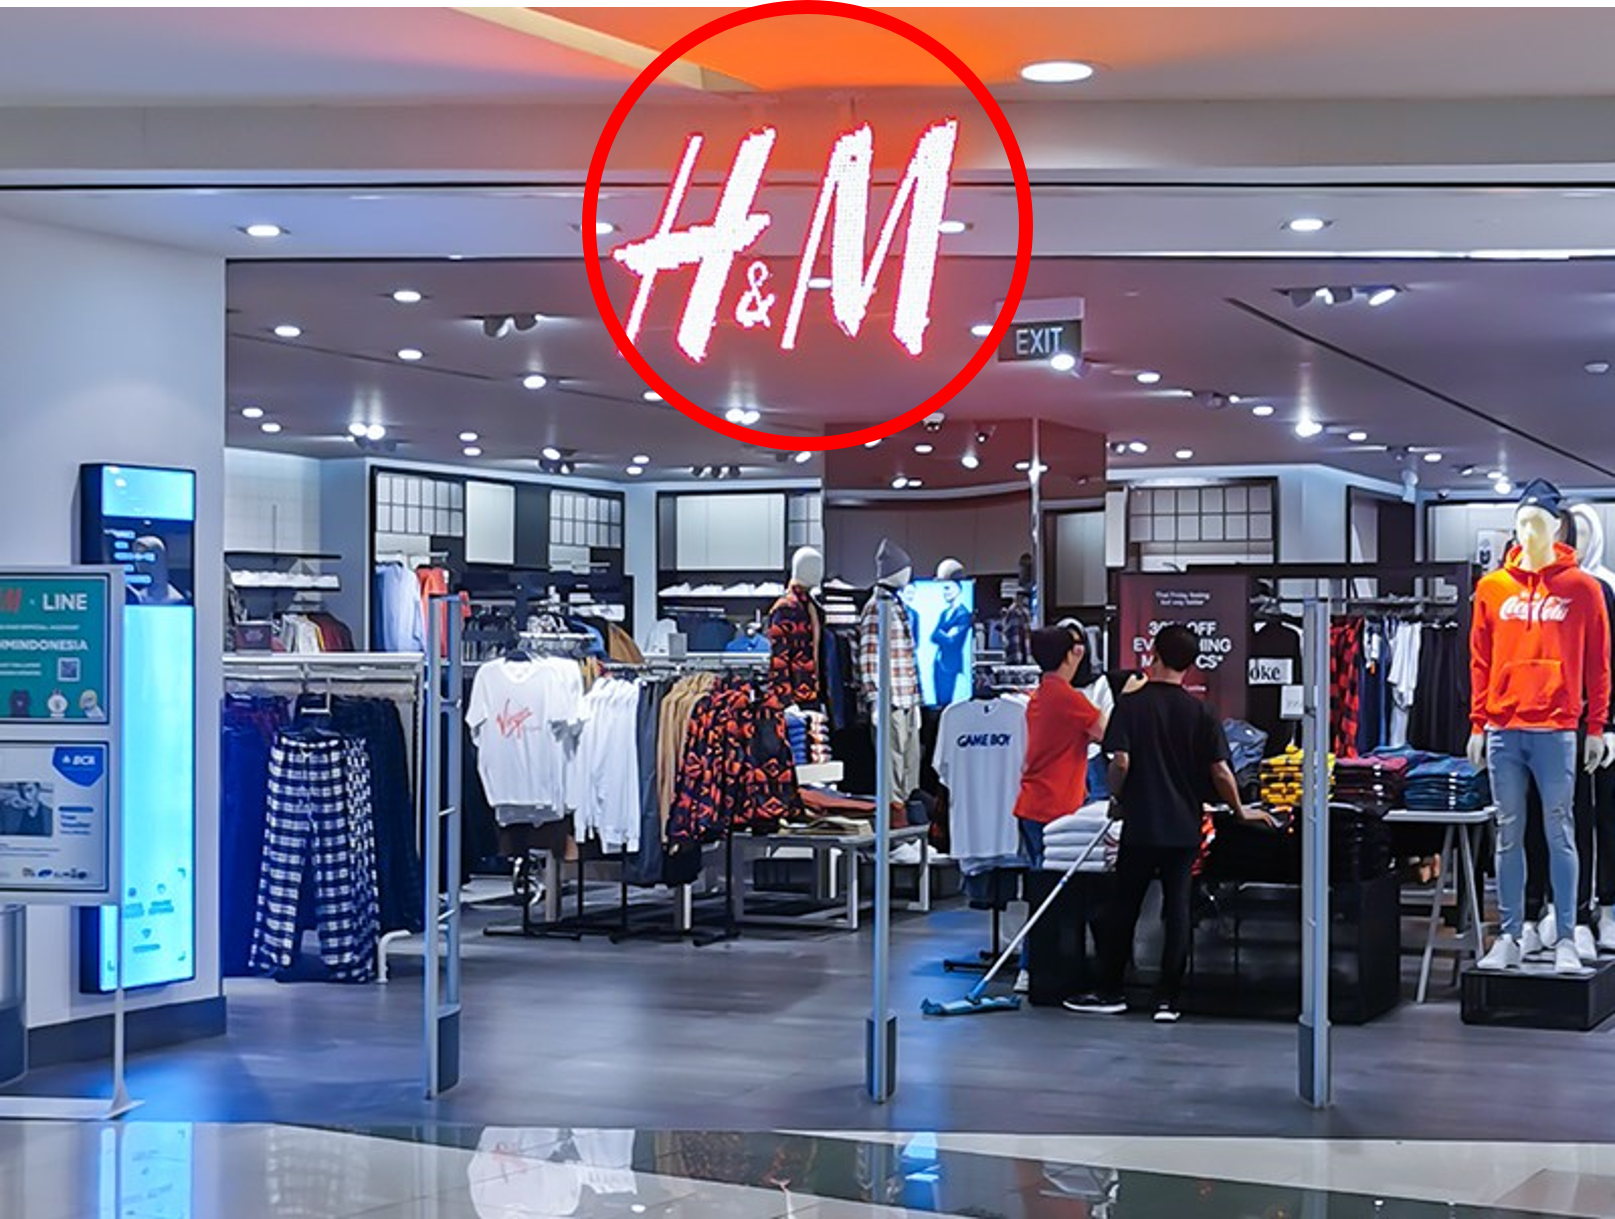
\includegraphics[width=0.35\linewidth]{hnm_circled.png}
	\caption{Contoh POI dengan logo unik.}
	\label{fig:poi_logo}
\end{figure}

\section{Object Instance Recognition}
\label{sec:oir}

\textit{Object Instance Recognition} (OIR) adalah teknik pengenalan objek spesifik. Pada teknik OIR deteksi tidak memberikan kelas dari gambar tetapi label yang khusus, seperti contohnya jika objek merupakan sebuah mobil, OIR tidak hanya akan memberikan keluaran bahwa objek merupakan mobil melainkan hal yang spesifik seperti merk dan jenis mobil tersebut. OIR bekerja dengan menerima gambar masukkan dan mencari gambar pada \textit{dataset} yang memiliki paling banyak kemiripan.

Penyelesaian OIR akan mudah bila gambar masukkan merupakan gambar yang sudah bersih. Pada praktiknya sebuah algoritma OIR seharusnya tetap dapat mengenali objek walaupun gambar bervariasi. Beberapa perubahan pada gambar berikut merupakan faktor-faktor yang dapat mempersulit proses OIR:
\begin{itemize}
	\item Cahaya \\
	Perubahan pada tingkat pencahayaan pada gambar yang mengakibatkan perubahan nilai \textit{pixel-pixel} pada gambar.
	\item Skala \\
	Jarak diambilnya gambar yang berisi objek. Perbedaan ukuran objek pada gambar akan menyebabkan sudut-sudut pada objek menjadi berbeda.
	\item Rotasi \\
	Orientasi atau arah pengambilan gambar yang berbeda akan mengakibatkan objek pada gambar jadi terlihat berbeda. Sudut-sudut akan menjadi berbeda karena arah hadapnya berbeda.
	\item Latar Belakang \\
	Objek-objek lain di sekitar objek yang ingin diidentifikasi akan berpotensi mempersulit pemrosesan. Objek-objek tersebut dapat menghasilkan fitur-fitur lokal yang tidak relevan terhadap objek yang ingin diidentifikasi.
	\item Bagian Objek Tertutup \\
	Adanya objek lain yang menutupi sebagian dari objek yang ingin diidentifikasi akan berpotensi menyebabkan beberapa fitur lokal dari objek tidak terdeteksi.
	\item Sudut Pandang \\
	Sudut pengambilan gambar yang berbeda akan memengaruhi pemrosesan. Fitur-fitur lokal dari objek yang ingin diidentifikasi akan menjadi berbeda.
	\item Translasi \\
	Posisi objek yang ingin diidentifikasi dalam gambar akan memengaruhi pemrosesan. Pencarian pasangan fitur lokal tidak dapat dengan hanya menggunakan posisi di mana fitur lokal tersebut ditemukan pada gambar.
\end{itemize}
\begin{figure}[H]
	\centering % <-- added
	\begin{subfigure}{0.3\textwidth}
		
\includegraphics[width=1\textwidth]{ideal.jpg}
		\caption{Gambar objek yang ideal, dari sudut tegak lurus}
		\label{fig:oir_ideal}
	\end{subfigure}\hfil % <-- added
	\begin{subfigure}{0.3\textwidth}
		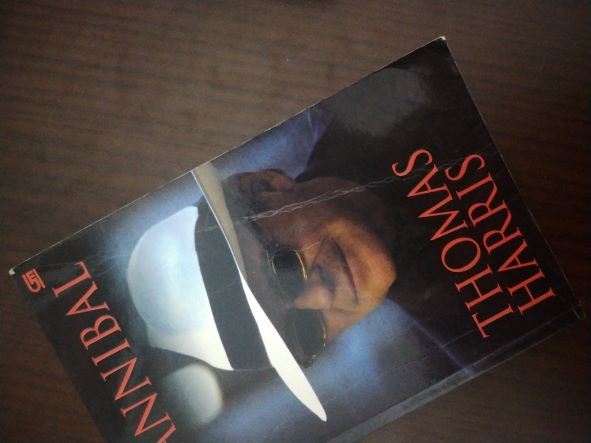
\includegraphics[width=1.33\textwidth, angle=270]{translasi.jpg}
		\caption{Objek pada gambar mengalami translasi dan rotasi}
		\label{fig:oir_translasi}
	\end{subfigure}\hfil % <-- added
	\begin{subfigure}{0.3\textwidth}
		
\includegraphics[width=1.33\textwidth, angle=270]{sudut.jpg}
		\caption{Gambar diambil dari sudut yang berbeda}
		\label{fig:oir_sudut}
	\end{subfigure}\hfill
	
	\medskip
	\begin{subfigure}{0.3\textwidth}
		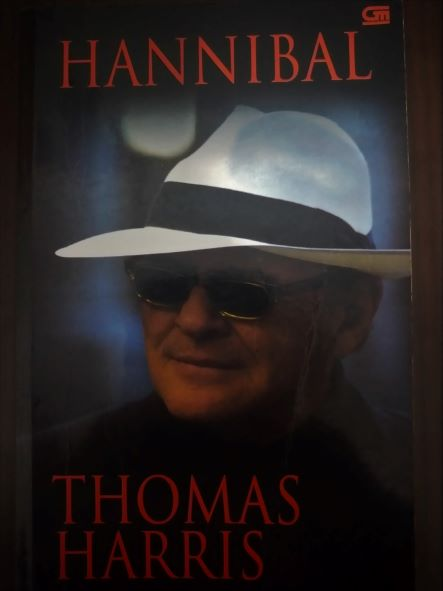
\includegraphics[width=\linewidth]{cahaya.jpg}
		\caption{Gambar dengan pencahayaan yang berbeda}
		\label{fig:oir_cahaya}
	\end{subfigure}\hfil % <-- added
	\begin{subfigure}{0.3\textwidth}
		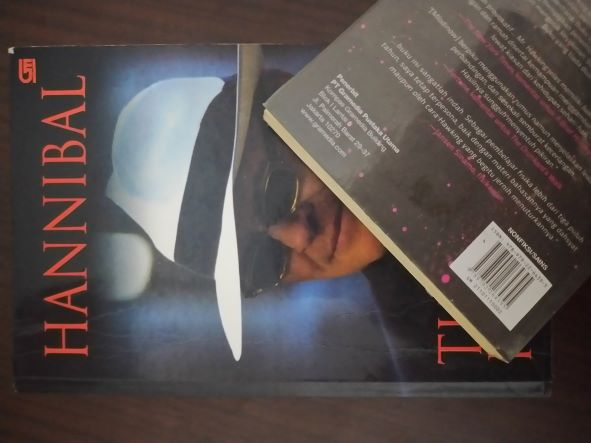
\includegraphics[width=1.33\textwidth, angle=270]{terhalang.jpg}
		\caption{Objek pada gambar terhalang oleh objek lain}
		\label{fig:oir_terhalang}
	\end{subfigure}\hfil % <-- added
	\begin{subfigure}{0.3\textwidth}
		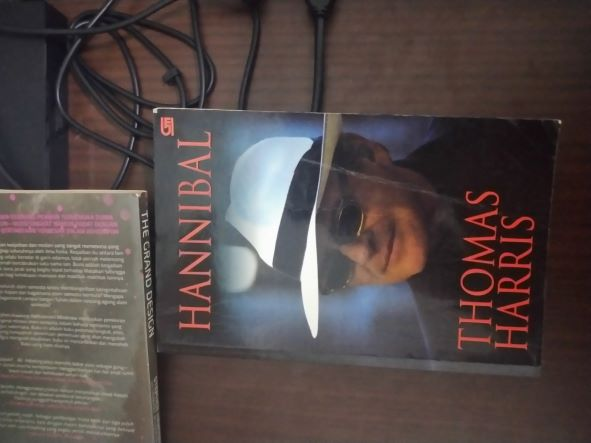
\includegraphics[width=1.33\textwidth, angle=270]{latar-belakang.jpg}
		\caption{Terdapat objek lain di latar belakang dari objek utama}
		\label{fig:oir_latar-belakang}
	\end{subfigure}
	\caption{Contoh variasi pada gambar \textit{cover} buku yang dapat menyebabkan masalah pada OIR}
	\label{fig:images}
\end{figure}

OIR dapat dilakukan dengan menggunakan fitur lokal. Fitur lokal sendiri merupakan fitur dalam gambar yang mendeskripsikan sebuah daerah tertentu pada gambar tersebut. Fitur lokal dapat berupa perpotongan garis atau yang biasa disebut \textit{keypoint}. Sebuah \textit{keypoint} akan dapat diidentifikasi dengan menggunakan daerah di sekitar \textit{keypoint} tersebut. Deskripsi \textit{keypoint} ini dibuat dalam sebuah vektor yang dinamakan vektor deskriptor.

Teknik OIR bekerja dengan melakukan deteksi fitur lokal pada gambar masukkan dan pada gambar-gambar di \textit{dataset}. Fitur-fitur lokal dari gambar masukkan tersebut kemudian dipasangkan dengan fitur lokal dari gambar \textit{dataset}. Gambar yang memiliki pasangan terbanyak akan merupakan hasil deteksi gambar masukkan tersebut. 

Pengambilan fitur lokal dari gambar dapat dilakukan dengan beberapa metode, seperti SIFT (lihat~\ref{sec:sift}) dan ORB (lihat~\ref{sec:orb}). Kedua metode tersebut---SIFT dan ORB---sudah menangani masalah perubahan translasi, skala dan rotasi karena fitur lokal yang dihasilkan oleh SIFT dan ORB bersifat invarian terhadap translasi, skala dan rotasi.

Proses pencarian pasangan fitur lokal dari gambar masukkan dan \textit{dataset} dilakukan dengan menggunakan vektor deskriptor dari fitur lokal. Perubahan-perubahan pada gambar walaupun sedikit akan menyebabkan perubahan nilai pada vektor deskriptor. Vektor deskriptor dari fitur lokal pada gambar masukkan hampir tidak akan persis sama dengan vektor deskriptor dari gambar yang ada di \textit{dataset}. Oleh karena itu pencarian pasangan fitur lokal dilakukan dengan mencari pasangan fitur lokal yang memiliki nilai kemiripan paling tinggi.

Secara garis besar tahapan proses OIR pada penelitian ini adalah sebagai berikut:
\begin{enumerate}
	\item Ekstraksi Fitur \\
	Pertama akan dilakukan pengambilan fitur-fitur lokal dari gambar masukkan. Dengan menggunakan metode SIFT atau ORB pengambilan fitur lokal akan menghasilkan \textit{tuple} yang  berisi \textit{keypoint}. Setiap \textit{keypoint} yang dihasilkan akan memiliki sebuah vektor yang akan digunakan untuk mengidentifikasi \textit{keypoint} tersebut. Vektor ini disebut sebagai vektor deskriptor.
	\item Pairing \\
	Untuk setiap fitur lokal yang terdeteksi pada gambar masukkan akan dicari beberapa fitur lokal dari gambar pada \textit{dataset} yang paling mirip. Kemiripan fitur lokal ditentukan dengan menghitung jarak (sesuai dengan metrik yang digunakan) antara vektor deskriptor dari kedua fitur lokal tersebut.
	\item Verification \\
	Pasangan fitur lokal yang didapat pada tahap sebelumnya merupakan pasangan yang hanya memiliki ciri yang mirip tetapi belum tentu konsisten secara geometris. Pasangan fitur lokal dikatakan konsisten secara geometris jika keduanya memiliki posisi yang sama relatif terhadap pasangan lain di sekitarnya. Penjelasan mengenai pasangan yang konsisten akan dijelaskan pada paragraf di bawah. Hanya pasangan-pasangan fitur lokal yang konsisten secara geometris yang akan diproses lebih lanjut.
	\item Scoring \\
	Setelah didapatkan semua pasangan fitur lokal yang paling mirip dan konsisten secara geometris maka dapat ditentukan pasangan gambar yang menjadi label gambar masukkan. Kemudian perlu dihitung nilai kemiripan dari label yang dihasilkan. Kemiripan dapat dihitung dengan menghitung $\frac{1}{d}$ untuk semua pasangan fitur lokal, di mana $d$ merupakan jarak pasangan tersebut. Nilai-nilai $\frac{1}{d}$ tersebut kemudian dihitung totalnya untuk menjadi nilai kemiripan label hasil.
\end{enumerate}
\begin{figure}[H]
	\begin{subfigure}[b]{.5\textwidth}
		\centering
		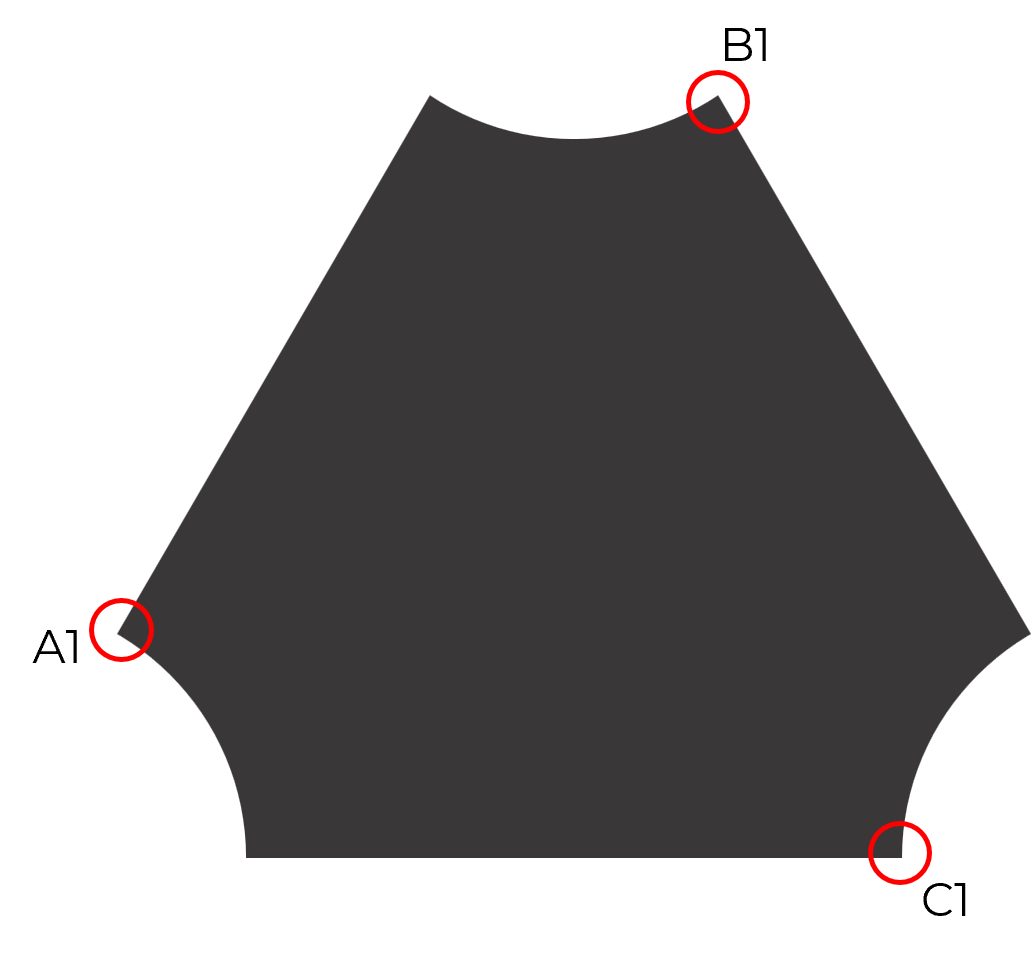
\includegraphics[width=0.7\linewidth]{geo_ver1.png}
		\caption{}
		\label{subfig:geo_ver1}
	\end{subfigure}%
	\begin{subfigure}[b]{.5\textwidth}
		\centering
		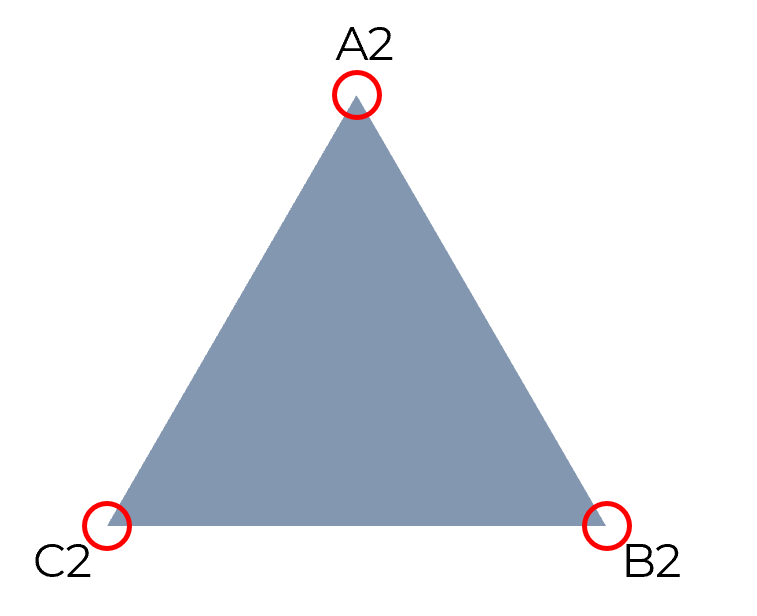
\includegraphics[width=0.7\linewidth]{geo_ver2.png}
		\caption{}
		\label{subfig:geo_ver2}
	\end{subfigure}
	\caption{Ilustrasi pasangan fitur lokal yang konsisten dan tidak konsisten.}
	\label{fig:geo_ver}
\end{figure}
Ilustrasi untuk menunjukkan pasangan yang tidak konsisten dapat dilihat pada Gambar~\ref{fig:geo_ver}. Pada kedua gambar tersebut, fitur lokal A1, B1, dan C1 pada Gambar~\ref{subfig:geo_ver1} secara berurutan dipasangkan dengan fitur lokal A2, B2, dan C2 pada Gambar~\ref{subfig:geo_ver2}. 

Pada orientasi seperti di gambar, pasangan A1 dengan A2 dan B1 dengan B2 merupakan pasangan yang tidak konsisten. Hal tersebut dikarenakan posisi A1 yang berada di sebelah kiri B1 tetapi pasangan dari A1, yaitu A2 berada di sebelah kiri pasangan dari B2, pasangan dari B1. Sedangkan pasangan C1 dengan C2 merupakan pasangan yang konsisten, karena baik C1 maupun C2 memiliki posisi relatif yang sama terhadap pasangan fitur lokal lain.

Gambar~\ref{subfig:geo_ver2} dapat dirotasi sebanyak 180 derajat sehingga B2 berada di sebelah kanan A1. Dengan menggunakan orientasi gambar yang seperti ini, pasangan A1 dengan A2 dan pasangan B1 dengan B2 menjadi konsisten posisinya secara geometris. Tetapi dengan orientasi yang seperti ini pasangan C1 dengan C2 menjadi tidak konsisten karena posisi C2 pada Gambar~\ref{subfig:geo_ver2} akan berada di sebelah kiri A2 dan B2.

Salah satu metode untuk melakukan verifikasi geometris adalah BSIS (lihat \ref{sec:bsis}). BSIS dapat mencari pasangan-pasangan fitur lokal yang posisi relatif konsisten terhadap pasangan lain. Verifikasi yang dilakukan BSIS dilakukan dengan menggunakan beberapa orientasi gambar untuk mendapatkan orientasi yang menghasilkan nilai kemiripan paling tinggi.

Cara lain yang dapat dilakukan pada tahap verifikasi adalah dengan melakukan \textit{Lowe's Ratio Test}. Cara ini tidak mencari pasangan yang konsisten secara geometris melainkan hanya menyaring pasangan yang kuat. \textit{Lowe's Ratio Test} mencari pasangan yang kuat dengan membandingkan kemiripan dua pasangan paling mirip untuk tiap fitur lokal di gambar masukkan. 

Untuk sebuah fitur lokal Q dari gambar masukkan dihitung nilai kemiripannya dengan setiap fitur lokal gambar \textit{dataset}, didapatkan fitur lokal T1 merupakan fitur lokal yang nilai kemiripannya paling tinggi dan T2 merupakan fitur lokal yang nilai kemiripannya kedua tertinggi. Pasangan fitur lokal Q dan T1 akan dikatakan pasangan yang jika nilai kemiripannya memenuhi persamaan berikut:
\begin{equation}
	similarity(Q, T1) > similarity(Q, T2) \times n
\end{equation}
Variabel $n$ pada persamaan di atas merupakan sebuah nilai konstan yang nilainya lebih dari 1. Persamaan tersebut bertujuan untuk mencari pasangan yang benar-benar mirip dan nilai kemiripannya berbeda jauh dengan pasangan lainnya. Nilai $n$ dapat diatur untuk menyatakan seberapa perlu seberapa jauh jarak pasangan termirip dengan kedua termirip.

\section{SIFT (Scale Invariant Feature Transform)}
\label{sec:sift}
SIFT adalah salah satu metode pencarian fitur lokal yang dicetuskan pada~\cite{lowe2004sift}. Fitur lokal yang dihasilkan SIFT bersifat invarian terhadap rotasi, perubahan skala, dan translasi pada gambar. Sifat invarian ini berarti fitur lokal yang sama pada gambar yang telah dirotasi, diubah skalanya, atau ditranslasi akan tetap memiliki ciri yang mirip. Setiap fitur lokal akan memiliki sebuah vektor yang mendeskripsikan daerah area fitur lokal tersebut, vektor ini biasa disebut sebagai deskriptor. Vektor deksriptor SIFT berbentuk vektor bilangan bulat yang memiliki 128 elemen. Tahap pencarian fitur lokal pada SIFT dapat dibagi menjadi 4 langkah yang akan dijabarkan pada subbab-subbab berikut.

\subsection{Pencarian Extrema}
Pada tahap ini akan dicari \textit{pixel-pixel} pada gambar yang merupakan \textit{corner} atau biasa disebut \textit{keypoint}. \textit{Keypoint} pada SIFT dicari dengan memeriksa \textit{pixel-pixel} pada gambar hasil turunan kedua Gaussian. Turunan kedua Gaussian akan dihitung dengan menggunakan \textit{Difference of Gaussian} (DoG).

Penghitungan DoG ini dilakukan dengan memanfaatkan sifat dari \textit{Matrix} Konvolusi Gaussian. \textit{Matrix} Konvolusi Gaussian merupakan \textit{matrix} yang memiliki sifat distribusi Gaussian, di mana titik tengah \textit{matrix} memiliki nilai yang tinggi dan nilai-nilai di sekitarnya semakin mengecil semakin mendekati tepi \textit{matrix}. Seperti ditunjukkan pada Gambar~\ref{fig:gaussian_function}. 

\begin{figure}[H]
	\begin{subfigure}[b]{.5\textwidth}
		\centering
		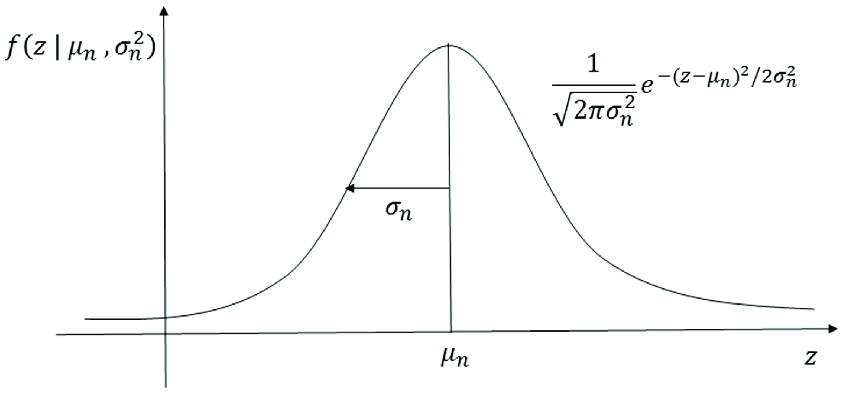
\includegraphics[width=1\linewidth]{gaussian_curve_s.png}
		\caption{}
		\label{subfig:gaussian_curve}
	\end{subfigure}%
	\begin{subfigure}[b]{.5\textwidth}
		\centering
		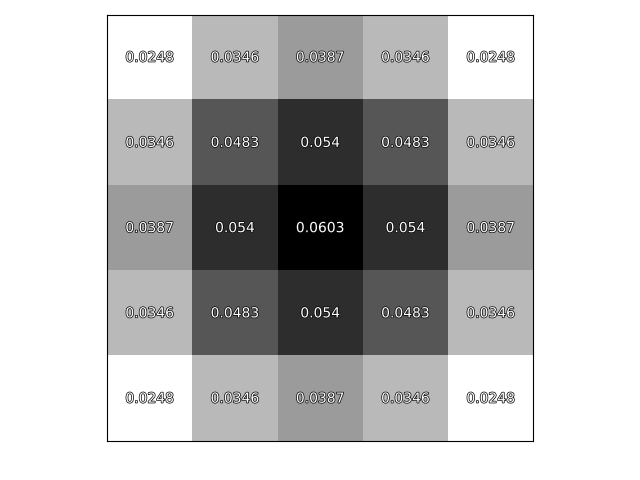
\includegraphics[width=0.9\linewidth]{gaussian_matrix_3.png}
		\caption{}
		\label{subfig:gaussian_matrix}
	\end{subfigure}
	\caption{Kurva Gaussian dan bentuk representasi \textit{matrix}-nya.}
	\label{fig:gaussian_function}
\end{figure}

Pada fungsi Gaussian tingkat penyebaran data dapat diatur dengan mengubah parameter $\sigma$ yang mengatur nilai deviasi standar. Gambar~\ref{subfig:gaussian_curve} menunjukkan bagaimana nilai $\sigma$ mengatur bagaimana data tersebar dari \textit{mean}, di mana semakin tinggi nilai $\sigma$ maka data akan semakin menyebar. Nilai yang semakin menyebar menyebabkan perbedaan nilai antar titik semakin kecil. Efeknya pada \textit{matrix} dapat dilihat pada Gambar~\ref{fig:gaussian_sigma}. Nilai $\sigma$ yang tinggi menyebabkan kurva semakin melebar dan pada \textit{matrix} selisih nilai antar titik menjadi semakin kecil.

\begin{figure}[H]
	\begin{subfigure}[b]{.5\textwidth}
		\centering
		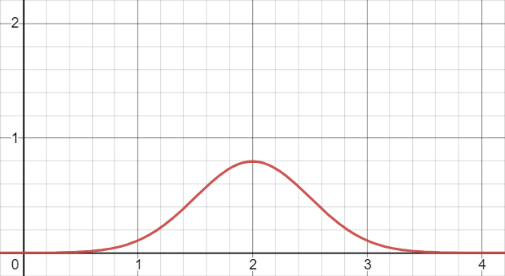
\includegraphics[width=0.9\linewidth]{gaussian_curve_1.png}
		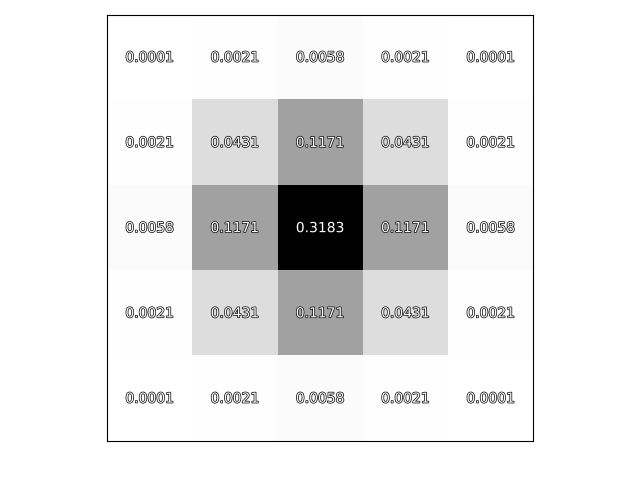
\includegraphics[width=0.9\linewidth]{gaussian_matrix_1.png}
		\caption{$\sigma=1$}
		\label{subfig:gaussian_sigma1}
	\end{subfigure}%
	\begin{subfigure}[b]{.5\textwidth}
		\centering
		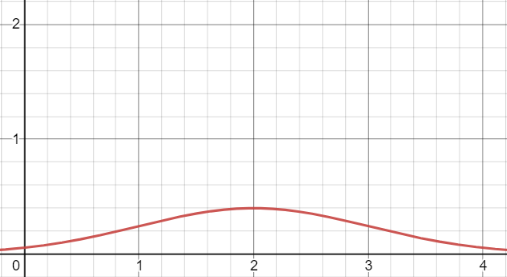
\includegraphics[width=0.9\linewidth]{gaussian_curve_2.png}
		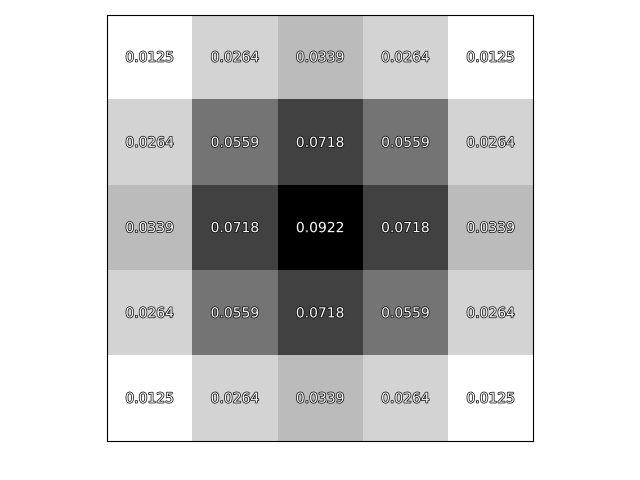
\includegraphics[width=0.9\linewidth]{gaussian_matrix_2.png}
		\caption{$\sigma=2$}
		\label{subfig:gaussian_sigma2}
	\end{subfigure}
	\caption{Kurva dan \textit{matrix} Gaussian pada nilai $\sigma$ yang berbeda.}
	\label{fig:gaussian_sigma}
\end{figure}

\textit{Matrix} Konvolusi Gaussian ketika diaplikasikan pada gambar akan menyebabkan perubahan nilai tiap \textit{pixel} pada gambar. Nilai dari setiap \textit{pixel} akan menjadi mirip dengan \textit{pixel} tetangga di dekatnya. Perubahan nilai \textit{pixel} akan paling berpengaruh pada daerah dengan perubahan nilai \textit{pixel} yang tinggi. Tingkat perubahan nilai dipengaruhi oleh nilai $\sigma$ yang digunakan, nilai $\sigma$ yang tinggi akan menyebabkan nilai \textit{pixel} yang berdekatan semakin mirip---perubahan nilai \textit{pixel} pada daerah tersebut semakin mengecil. Jika dilihat pada gambar, maka gambar hasil konvolusi akan terlihat kabur (\textit{blur}). Nilai $\sigma$ menentukan tingkat \textit{blur} gambar.

\begin{figure}[H]
	\centering
	\begin{subfigure}[b]{.33\textwidth}
		\centering
		
\includegraphics[width=0.9\linewidth]{1.0_asus_logo2.jpeg}
		\caption{$\sigma=1.0$}
		\label{subfig:asus_sigma1.0}
	\end{subfigure}%
	\begin{subfigure}[b]{.33\textwidth}
		\centering
		
\includegraphics[width=0.9\linewidth]{1.4_asus_logo2.jpeg}
		\caption{$\sigma=1.4$}
		\label{subfig:asus_sigma1.4}
	\end{subfigure}
	\begin{subfigure}[b]{.33\textwidth}
		\centering
		
\includegraphics[width=0.9\linewidth]{1.8_asus_logo2.jpeg}
		\caption{$\sigma=1.8$}
		\label{subfig:asus_sigma1.8}
	\end{subfigure}
	\caption{Efek nilai $\sigma$ pada hasil gambar konvolusi.}
	\label{fig:asus_konv}
\end{figure}

Perubahan nilai $\sigma$ pada \textit{matrix} konvolusi serta efeknya pada gambar akan dimanfaatkan untuk menghitung \textit{Difference of Gaussian} (DoG). DoG merupakan hasil turunan kedua Gaussian pada gambar. Gambar DoG dapat diperoleh dengan menghitung perbedaan nilai tiap \textit{pixel} dari dua gambar yang telah dikonvolusi oleh \textit{matrix} Gaussian dengan nilai $\sigma$ yang berbeda. Perbedaan nilai untuk DoG dihitung dengan mengurangi setiap \textit{pixel} pada gambar konvolusi yang memiliki nilai $\sigma$ yang lebih kecil, dengan setiap \textit{pixel} pada posisi yang sama pada gambar konvolusi yang memiliki nilai $\sigma$ yang lebih besar. Ilustrasi dapat dilihat pada Gambar~\ref{fig:dog_asus}. 
\begin{figure}[H]
	\centering
	\includegraphics[width=\linewidth]{asus_dog.png}
	\caption{Operasi DoG pada gambar}
	\label{fig:dog_asus}
\end{figure} 

Metode SIFT mencari \textit{keypoint} dengan memanfaatkan konsep DoG. Sebuah gambar akan dikonvolusi dengan \textit{matrix} Gaussian beberapa kali dengan nilai $\sigma$ yang berbeda. Setelah didapatkan beberapa gambar maka akan dihitung DoG untuk setiap gambar yang nilai $\sigma$-nya bersebelahan (Gambar~\ref{fig:dog_scales}). Pasangan gambar konvolusi yang berbeda akan menghasilkan gambar DoG yang berbeda juga.  

Untuk setiap gambar DoG akan ditentukan \textit{pixel} mana saja yang merupakan \textit{keypoint} dengan mencari \textit{pixel} yang merupakan \textit{extrema}. Sebuah \textit{pixel} merupakan \textit{extrema} jika nilai pixel tersebut lebih besar dari seluruh 26 \textit{pixel} di sekitarnya atau lebih kecil dari seluruhnya. Ke-26 \textit{pixel} tersebut merupakan 8 \textit{pixel} yang mengelilingi, 9 \textit{pixel} pada posisi yang sama dari gambar di atasnya, dan juga 9 \textit{pixel} pada posisi yang sama dari gambar di bawahnya.
\begin{figure}[H]
	\centering
	\includegraphics[width=0.7\linewidth]{dog_scales.png}
	\caption{Penggunaan DoG pada SIFT}
	\label{fig:dog_scales}
\end{figure} 

\newpage
\subsection{Penentuan Skala}
Pada tahap sebelumnya sudah didapatkan \textit{keypoint-keypoint} dalam gambar. Agar \textit{keypoint} dapat invarian terhadap skala, \textit{keypoint} perlu untuk dapat tetap terdeteksi walaupun ukuran gambar berubah. Untuk setiap \textit{keypoint} perlu untuk dicari skala terkecil di mana \textit{keypoint} tersebut dapat terdeteksi. Untuk mencapai ini SIFT menggunakan lanjutan dari metode pada Gambar~\ref{fig:dog_scales} dengan langkah sebagai berikut (ilustrasi pada Gambar~\ref{fig:oktaf}):
\begin{enumerate}
	\item Lakukan konvolusi sampai nilai $\sigma$ sudah mencapai 2 kali nilai awal
	\item Perkecil ukuran gambar (\textit{downsample}) menjadi setengah resolusinya
	\item Kembalikan nilai $\sigma$ ke nilai awal
	\item Ulang tahap dari langkah 1 hingga gambar sudah terlalu kecil.
\end{enumerate}

Pada langkah di atas setiap siklus ukuran gambar disebut sebagai oktaf, dimulai dari oktaf pertama, lalu kedua, dan seterusnya. Dengan setiap oktaf ukuran gambar akan semakin kecil. Pencarian \textit{keypoint} dilakukan pada tiap oktaf, dan untuk tiap \textit{keypoint} tersebut ditulis nilai oktaf tertinggi (ukuran gambar terkecil) di mana \textit{keypoint} tersebut dapat terdeteksi.

\begin{figure}[H]
	\centering
	\includegraphics[width=0.6\linewidth]{oktaf.png}
	\caption{Oktaf pada proses konvolusi SIFT}
	\label{fig:oktaf}
\end{figure}

\subsection{Penentuan Orientasi}
Untuk dapat invarian terhadap rotasi gambar, setiap \textit{keypoint} perlu memiliki orientasi yang konsisten. Untuk mendapatkan orientasi yang sama pada setiap rotasi gambar, orientasi perlu ditentukan dari atribut yang akan selalu sama bagaimanapun gambar dirotasi. Untuk itu orientasi \textit{keypoint} ditentukan dengan menggunakan orientasi yang dominan dari \textit{pixel-pixel} di sekitar \textit{keypoint}. Luas daerah yang digunakan untuk mendapat orientasi ditentukan oleh skala dari \textit{keypoint}. 

Penentuan orientasi yang dominan dihitung dengan menggunakan \textit{magnitude} ($m(x,y)$) dan orientasi ($\theta(x,y)$) dari \textit{pixel-pixel} dengan menggunakan rumus pada Persamaan~\ref{eq:magnitude} dan Persamaan~\ref{eq:orientasi}. $L(x,y)$ pada kedua persamaan tersebut merupakan gambar hasil konvolusi.
\begin{equation}
	\label{eq:magnitude}
	m(x,y)=\sqrt{(L(x+1,y)-L(x-1,y))^{2}+L(x,y+1)-L(x,y+1))^{2}}
\end{equation}
\begin{equation}
	\label{eq:orientasi}
	\theta(x,y)=\tan^{-1}((L(x,y+1)-L(x,y-1))/(L(x+1,y)-L(x-1,y)))
\end{equation}
Setiap \textit{pixel} akan dihitung orientasi dan \textit{magnitude}-nya. \textit{Magnitude} akan digunakan sebagai bobot dari \textit{pixel} tersebut. Selain \textit{magnitude}, bobot sebuah \textit{pixel} juga dipengaruhi oleh \textit{Gaussian Weighting}, yang membuat \textit{pixel} yang posisinya dekat dengan titik pusat (titik \textit{keypoint}) akan memiliki bobot yang lebih tinggi dibanding yang lokasinya jauh dari titik pusat. Ilustrasi pada Gambar~\ref{fig:gaussian_weighting} menunjukkan bagaimana pembobotan dihitung, \textit{pixel-pixel} yang berada dekat dengan \textit{keypoint} (titik tengah) akan diberi bobot yang lebih besar---ditandai dengan lingkaran yang tebal. Sedangkan bobot akan semakin berkurang untuk \textit{pixel} yang jauh dari \textit{keypoint}.

\begin{figure}[H]
	\centering
	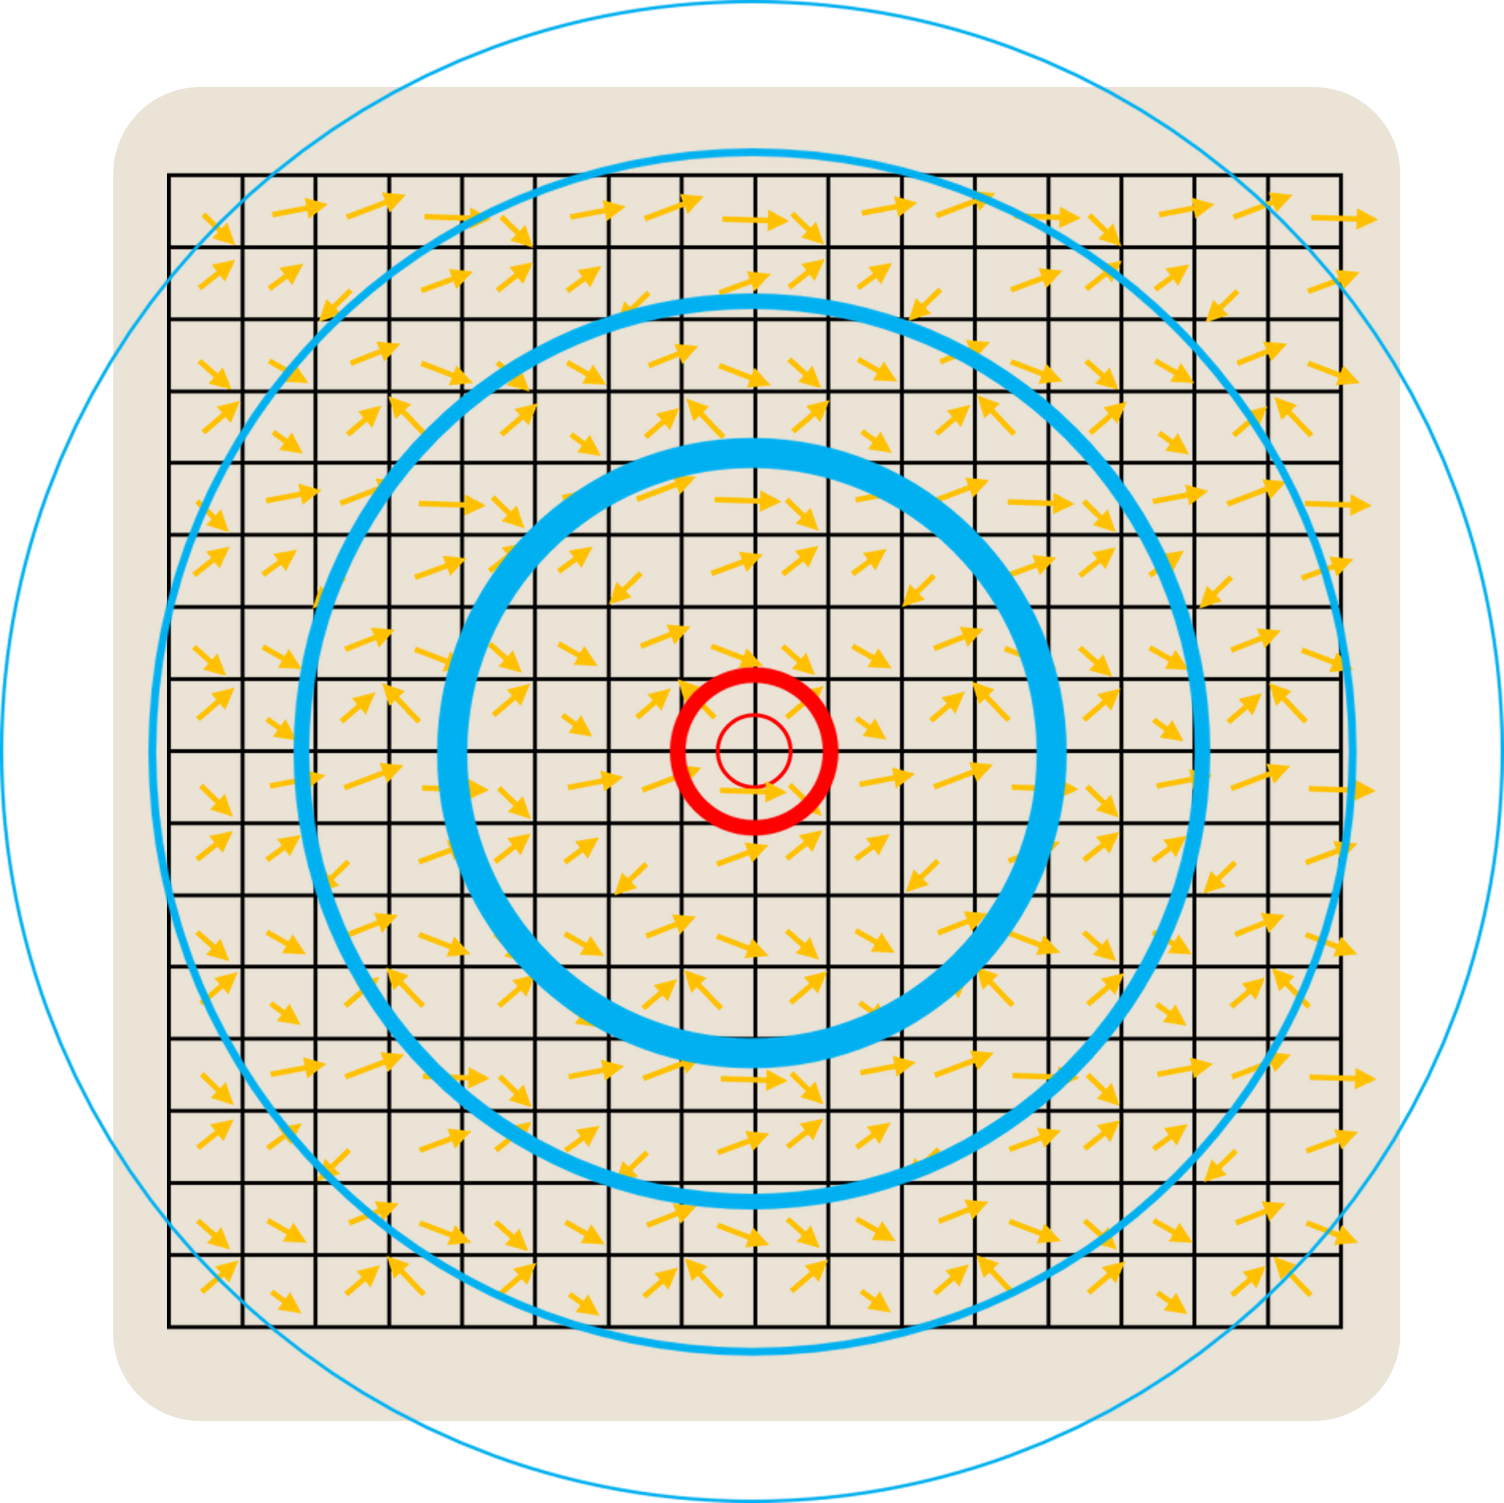
\includegraphics[width=0.45\linewidth]{gaussian_weighting.png}
	\caption{Ilustrasi pembobotan pada \textit{Gaussian Weighting}. Titik tengah merupakan \textit{keypoint} yang diperiksa sedangkan setiap kotak merupakan \textit{pixel-pixel} di sekitar \textit{keypoint}. Tanda panah pada tiap kotak menunjukkan \textit{magnitude} dan orientasi \textit{pixel} tersebut, panjang panah merupakan nilai \textit{magnitude} dan arahnya merupakan orientasi}
	\label{fig:gaussian_weighting}
\end{figure} 

Setelah setiap \textit{pixel} sudah dihitung orientasi dan bobotnya menggunakan \textit{magnitude} dan \textit{Gaussian Weighting}, nilai bobot tersebut akan dimasukkan ke dalam histogram berdasarkan orientasinya. Histogram yang digunakan memiliki 36 bin yang masing-masing mewakili 10 derajat orientasi. Ilustrasi dapat dilihat pada Gambar~\ref{fig:hist_orientasi}.
\begin{figure}[H]
	\centering
	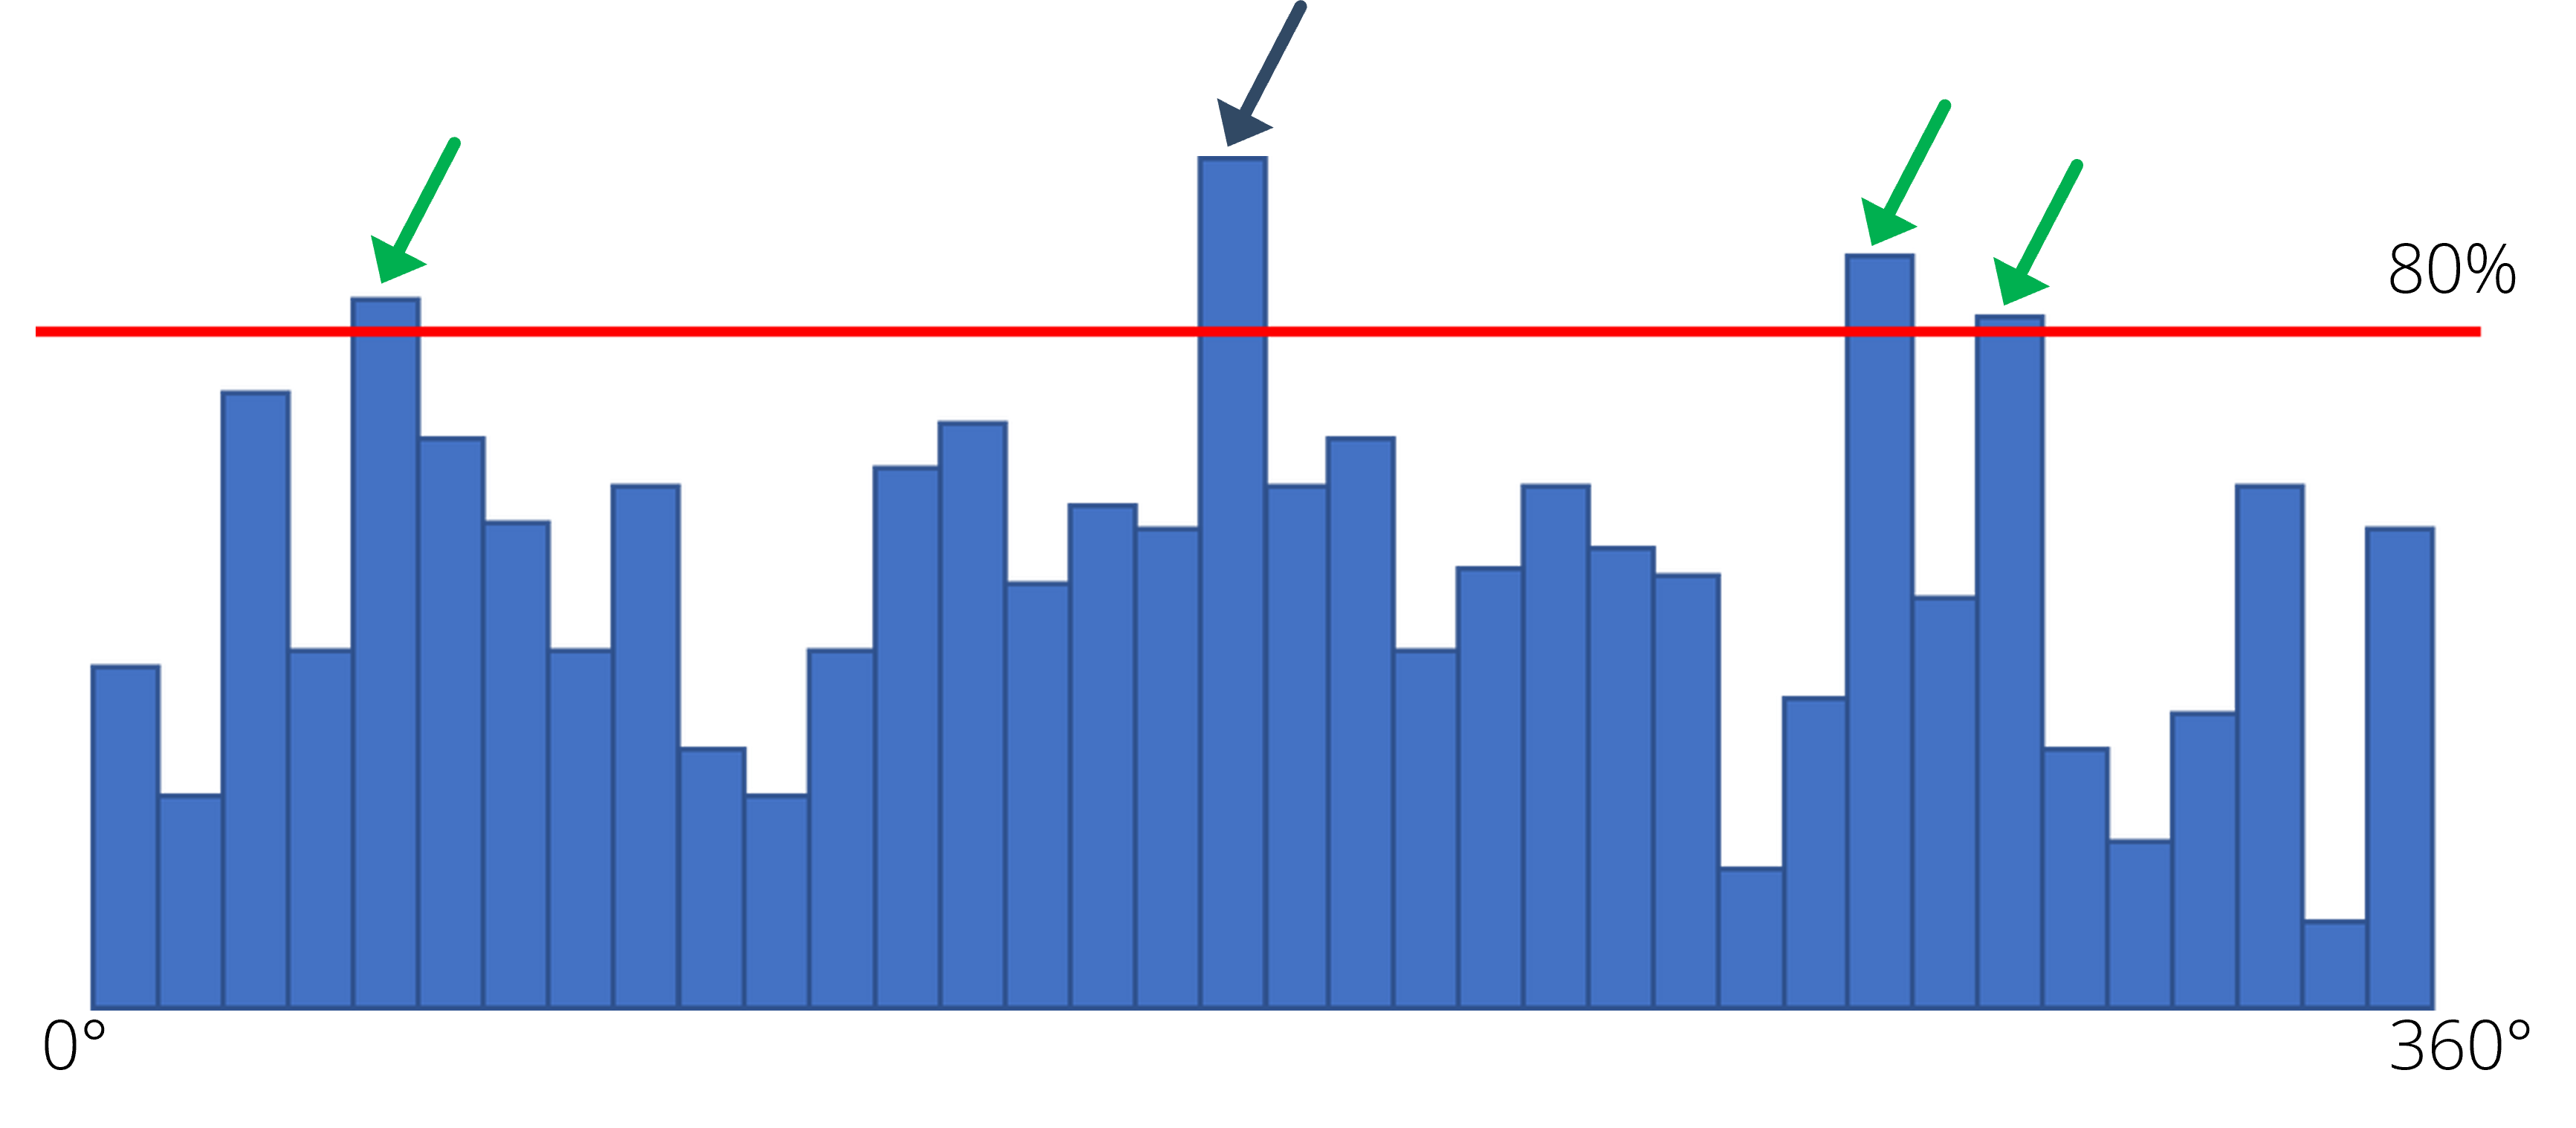
\includegraphics[width=0.8\linewidth]{hist_orientasi.png}
	\caption{Histogram untuk menentukan orientasi dari \textit{keypoint}. Bin dengan nilai tertinggi (tanda panah biru) akan digunakan sebagai orientasi dari \textit{keypoint}. Untuk bin lain yang jumlahnya berada dalam rentang $80\%$ dari bin tertinggi (tanda panah hijau) digunakan untuk membuat \textit{keypoint baru}.}
	\label{fig:hist_orientasi}
\end{figure}

Dari histogram tersebut puncak nilai bin tertinggi akan digunakan sebagai orientasi dari \textit{keypoint}. Untuk puncak-puncak lain yang berada dalam rentang $80\%$ dari puncak tertinggi akan digunakan untuk membuat \textit{keypoint} baru pada lokasi yang sama dengan orientasi yang berbeda sesuai dengan nilai orientasi pada bin tersebut.

\subsection{Pembuatan Deskriptor}
Setelah didapatkan \textit{keypoint} beserta skala dan orientasinya, perlu untuk diberikan sebuah identitas pada setiap \textit{keypoint}. Pemberian identitas ini berguna untuk mengidentifikasi \textit{keypoint} yang satu dengan yang lainnya, agar dapat ditemukan \textit{keypoint-keypoint} dengan ciri yang mirip. Identifikasi \textit{keypoint} dapat dilakukan dengan membuat sebuah vektor deskriptor. Vektor deskriptor merupakan vektor yang mendeskripsikan daerah di sekitar \textit{keypoint}. Vektor deskriptor pada SIFT berbentuk vektor berjumlah 128 elemen bilangan bulat.

Pembuatan vektor dilakukan dengan mengambil daerah di sekitar \textit{keypoint} dari gambar yang terlebih dahulu dirotasi sesuai dengan orientasi \textit{keypoint}. Ukuran daerah tersebut ditentukan berdasarkan dari skala \textit{keypoint}. Daerah tersebut kemudian dibagi menjadi $4\times4$ subdaerah. Untuk setiap subdaerah dihitung nilai \textit{magnitude} dan orientasi setiap \textit{pixel}-nya dengan diberi bobot menggunakan \textit{Gaussian Weighting} lalu hasilnya dimasukkan ke dalam histogram dengan 8 bin. Setiap bin dalam histogram mewakili 45 derajat orientasi. Nilai dari setiap bin pada histogram akan menjadi satu elemen pada deskriptor. Terdapat total 16 subdaerah dengan setiap daerah menghasilkan 8 elemen, sehingga didapat total sebanyak $16\times8=128$ elemen untuk vektor deskriptor. 

\subsection{SIFT di OpenCV}
\textit{Library} OpenCV di Python memiliki modul implementasi SIFT. Modul dapat digunakan untuk melakukan ekstraksi fitur lokal dari gambar dan menghasilkan vektor deskriptor untuk tiap fitur lokal. Untuk melakukan deteksi fitur lokal, pertama perlu untuk dibuat objek SIFT dengan menggunakan fungsi \texttt{SIFT\_create}. Beberapa parameter dari fungsi \texttt{SIFT\_create} yang relevan terhadap skripsi ini adalah sebagai berikut:
\begin{itemize}
	\item \texttt{nfeatures}: jumlah fitur yang ingin dihasilkan. Dipilih berdasarkan skor yang didapat dari nilai kontras pada daerah sekitar \textit{keypoint}.
	\item \texttt{nOctaveLayers}: jumlah lapisan untuk tiap oktaf. Ditentukan secara otomatis dari resolusi gambar.
	\item \texttt{sigma}: nilai $\sigma$ Gaussian yang digunakan pada oktaf pertama.
\end{itemize}

Objek SIFT tersebut lalu digunakan untuk mendeteksi fitur lokal dengan menggunakan fungsi \texttt{detectAndCompute}. Fungsi \texttt{detectAndCompute} menerima beberapa parameter berikut:
\begin{itemize}
	\item \texttt{image}: gambar masukkan yang ingin dideteksi \textit{keypoint}-nya. Berbentuk \textit{array} 2 dimensi.
	\item \texttt{mask}: \textit{array} 2 dimensi dengan ukuran yang sama dengan gambar, menentukan \textit{pixel} mana yang digunakan dan yang tidak.
\end{itemize}

Fungsi \texttt{detectAndCompute} tersebut akan menghasilkan sebuah \textit{tuple} yang berisi objek \textit{keypoint} dan \textit{array} berjumlah 128 elemen sebanyak \textit{keypoint} yang terdeteksi. Objek \textit{keypoint} yang dihasilkan memiliki atribut sebagai berikut:
\begin{itemize}
	\item \textbf{pt}: atribut ini memiliki dua buah atribut \textbf{x} dan \textbf{y} yang menunjukkan koordinat dari \textit{keypoint}.
	\item \textbf{size}: diameter daerah di sekitar \textit{keypoint} yang diperiksa.
	\item \textbf{angle}: orientasi dari \textit{keypoint}.
	\item \textbf{octave}: oktaf di mana \textit{keypoint} tersebut didapat.
\end{itemize} 

\section{ORB (Oriented FAST and Rotated BRIEF)}
\label{sec:orb}
ORB adalah metode pencarian fitur lokal yang dijelaskan pada~\cite{rublee2011orb}. ORB dapat menemukan fitur lokal dengan lebih cepat jika dibandingkan dengan SIFT, walaupun fitur lokal yang dihasilkan tidak seakurat yang dihasilkan SIFT. ORB mencari fitur lokal dengan mencari \textit{pixel} yang merupakan sudut perpotongan garis (\textit{Keypoint}). \textit{Keypoint} dalam ORB dicari dengan ide bahwa sebuah \textit{pixel} yang merupakan sudut akan memiliki garis kontinu membentuk lingkaran di sekitarnya dengan nilai intensitas yang lebih kecil atau lebih besar dari nilai intensitas \textit{pixel} tersebut. Fitur lokal yang dihasilkan ORB bersifat invarian terhadap rotasi, translasi dan invarian sebagian terhadap skala. Fitur lokal ORB juga memiliki sebuah vektor deskriptor yang berbentuk vektor sebanyak 256 elemen bilangan biner. Tahap pencarian fitur lokal pada ORB dibagi menjadi 4 langkah yang dijelaskan pada subbab-subbab berikut.

\subsection{Pencarian Keypoint}
\label{subsec:orb_keypoint}
Untuk menentukan apakah sebuah \textit{pixel} dalam gambar merupakan \textit{keypoint}, ORB mengambil nilai \textit{pixel} tersebut dan 16 \textit{pixel} di sekitarnya yang membentuk lingkaran. Dari ke 16 \textit{pixel} tersebut dibandingkan nilai intensitasnya dengan nilai intensitas \textit{pixel} yang berada di tengah ($p$), yaitu \textit{pixel} yang ingin diperiksa apakah merupakan \textit{keypoint}. Sebuah \textit{pixel} merupakan \textit{keypoint} jika dari 16 \textit{pixel} di sekitarnya terdapat setidaknya $n$ \textit{pixel} kontinu yang nilai intensitasnya lebih besar dari nilai $p + t$ atau lebih kecil dari $p - t$. Proses ini diilustrasikan pada Gambar~\ref{fig:orb_keypoint}

\begin{figure}[H]
	\centering
	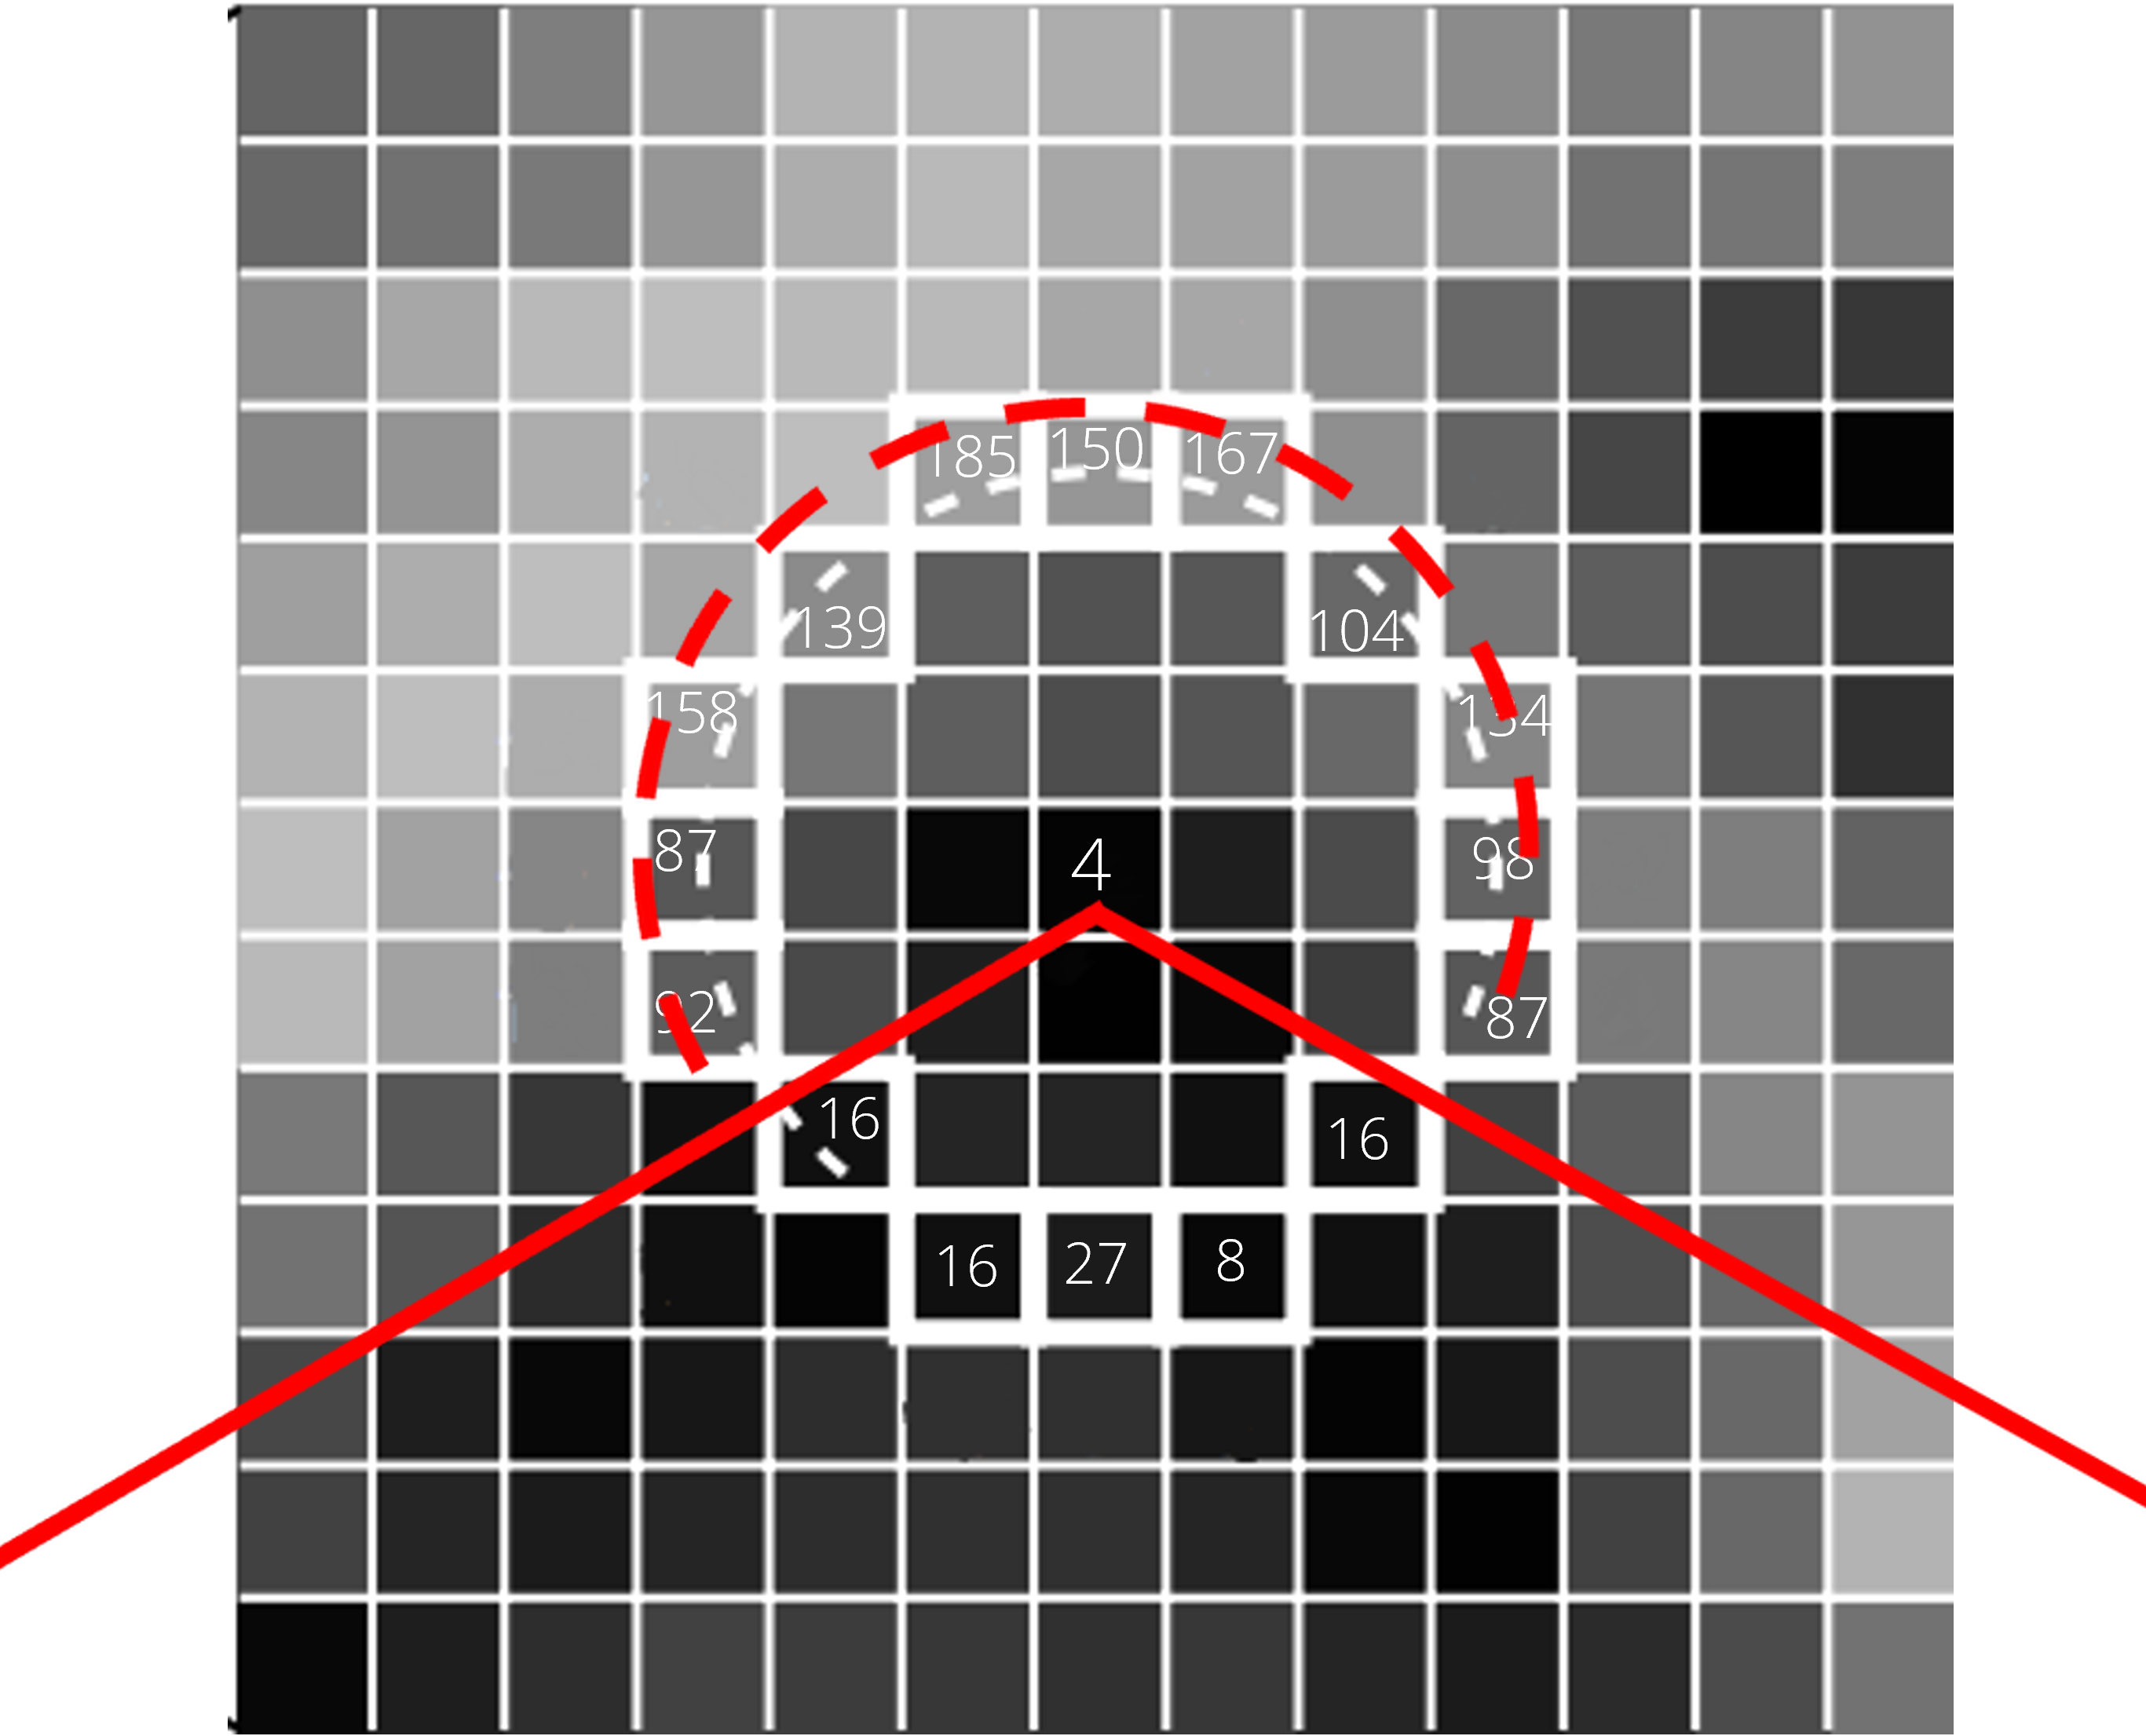
\includegraphics[width=0.5\linewidth]{orb_keypoint.png}
	%	\caption{Ilustrasi \textit{keypoint} pada ORB. Titik tengah pada gambar tersebut memiliki \textit{pixel-pixel} dengan nilai jauh lebih kecil (lebih gelap) yang mengelilinginya. \textit{Pixel-pixel} yang mengelilingi tersebut seakan membentuk sudut dengan titik tengah sebagai pusatnya.}
	\caption{Ilustrasi penentuan \textit{keypoint} pada ORB. Setiap kotak menunjukkan sebuah \textit{pixel} pada gambar dan angka di dalamnya merupakan nilai intensitasnya. \textit{Pixel} di tengah gambar (\textit{pixel} bernilai 4) merupakan \textit{pixel} yang akan diperiksa apakah merupakan \textit{keypoint}. \textit{Pixel-pixel} yang ditandai dengan kotak putih merupakan 16 \textit{pixel} yang digunakan untuk memeriksa apakah \textit{pixel} di tengah merupakan \textit{keypoint}.}
	\label{fig:orb_keypoint}	
\end{figure}

Pada ilustrasi di Gambar~\ref{fig:orb_keypoint} \textit{pixel} bernilai 4 yang berada di tengah gambar dapat menjadi \textit{keypoint} tergantung dari parameter $n$ dan $t$ yang digunakan. Di sekitar \textit{pixel} tersebut terdapat 11 \textit{pixel} kontinu yang nilai intensitasnya lebih besar setidaknya 83 satuan dari nilai intensitas \textit{pixel} tersebut.

\textit{Keypoint-keypoint} yang dihasilkan pada tahap ini belum tentu merupakan sebuah \textit{corner}. Metode yang digunakan ORB akan mendeteksi sebuah titik terang yang dikelilingi lingkaran dengan titik gelap atau sebaliknya menjadi sebuah \textit{keypoint}. Untuk itu perlu untuk disaring untuk mendapatkan hanya \textit{keypoint} yang merupakan \textit{corner}. 

Penentuan apakah \textit{keypoint} merupakan \textit{corner} pada ORB dilakukan dengan menggunakan \textit{Harris Corner Measure}. \textit{Harris Corner Measure} akan memberikan sebuah skor untuk sebuah daerah di sekitar \textit{pixel} untuk menunjukkan seberapa daerah tersebut merupakan \textit{corner}. 

\textit{Harris Corner Measure} menentukan apakah sebuah daerah merupakan \textit{corder} dengan menggunakan sebuah \textit{window} yang terpusat pada titik \textit{keypoint}. \textit{Window} tersebut lalu digerakkan ke beberapa arah dan dihitung intensitasnya untuk tiap pergerakan. Daerah tersebut merupakan \textit{corner} jika terdapat perubahan nilai intensitas ke arah manapun \textit{window} tersebut digerakkan.

Teknik \textit{Harris Corner Measure} akan menghasilkan sebuah skor $M$ yang menunjukkan nilai seberapa daerah yang diperiksa merupakan \textit{corner}. ORB akan mengambil $N$ \textit{keypoint} dengan nilai $M$ tertinggi untuk ditentukan sebagai \textit{keypoint}.  

\subsection{Penentuan Skala}
\label{subsec:orb_skala}
\textit{Keypoint} yang telah dideteksi pada tahap awal perlu untuk dapat terdeteksi juga walaupun ukuran gambar berubah agar sifatnya invarian terhadap skala. \textit{Keypoint} yang invarian terhadap skala adalah \textit{keypoint} dengan ciri yang tetap walaupun dideteksi pada ukuran gambar yang berbeda. 

Untuk mencapai sifat ini ORB menggunakan metode \textit{Image Pyramid}. ORB menggunakan \textit{Image Pyramid} dengan cara memperkecil ukuran gambar beberapa kali dan untuk setiap ukuran gambar dilakukan deteksi untuk \textit{keypoint}. Dengan menggunakan cara ini \textit{keypoint} tidak akan benar-benar invarian terhadap perubahan skala, \textit{keypoint} hanya invarian terhadap beberapa skala gambar yang digunakan pada \textit{pyramid}.

Ilustrasi dapat dilihat pada Gambar~\ref{fig:orb_pyramid}. Pada ilustrasi tersebut gambar awal diperkecil beberapa kali dengan membagi panjang dan lebarnya menjadi setengahnya. Untuk setiap ukuran gambar dicari \textit{keypoint-keypoint}-nya.

\begin{figure}[H]
	\centering
	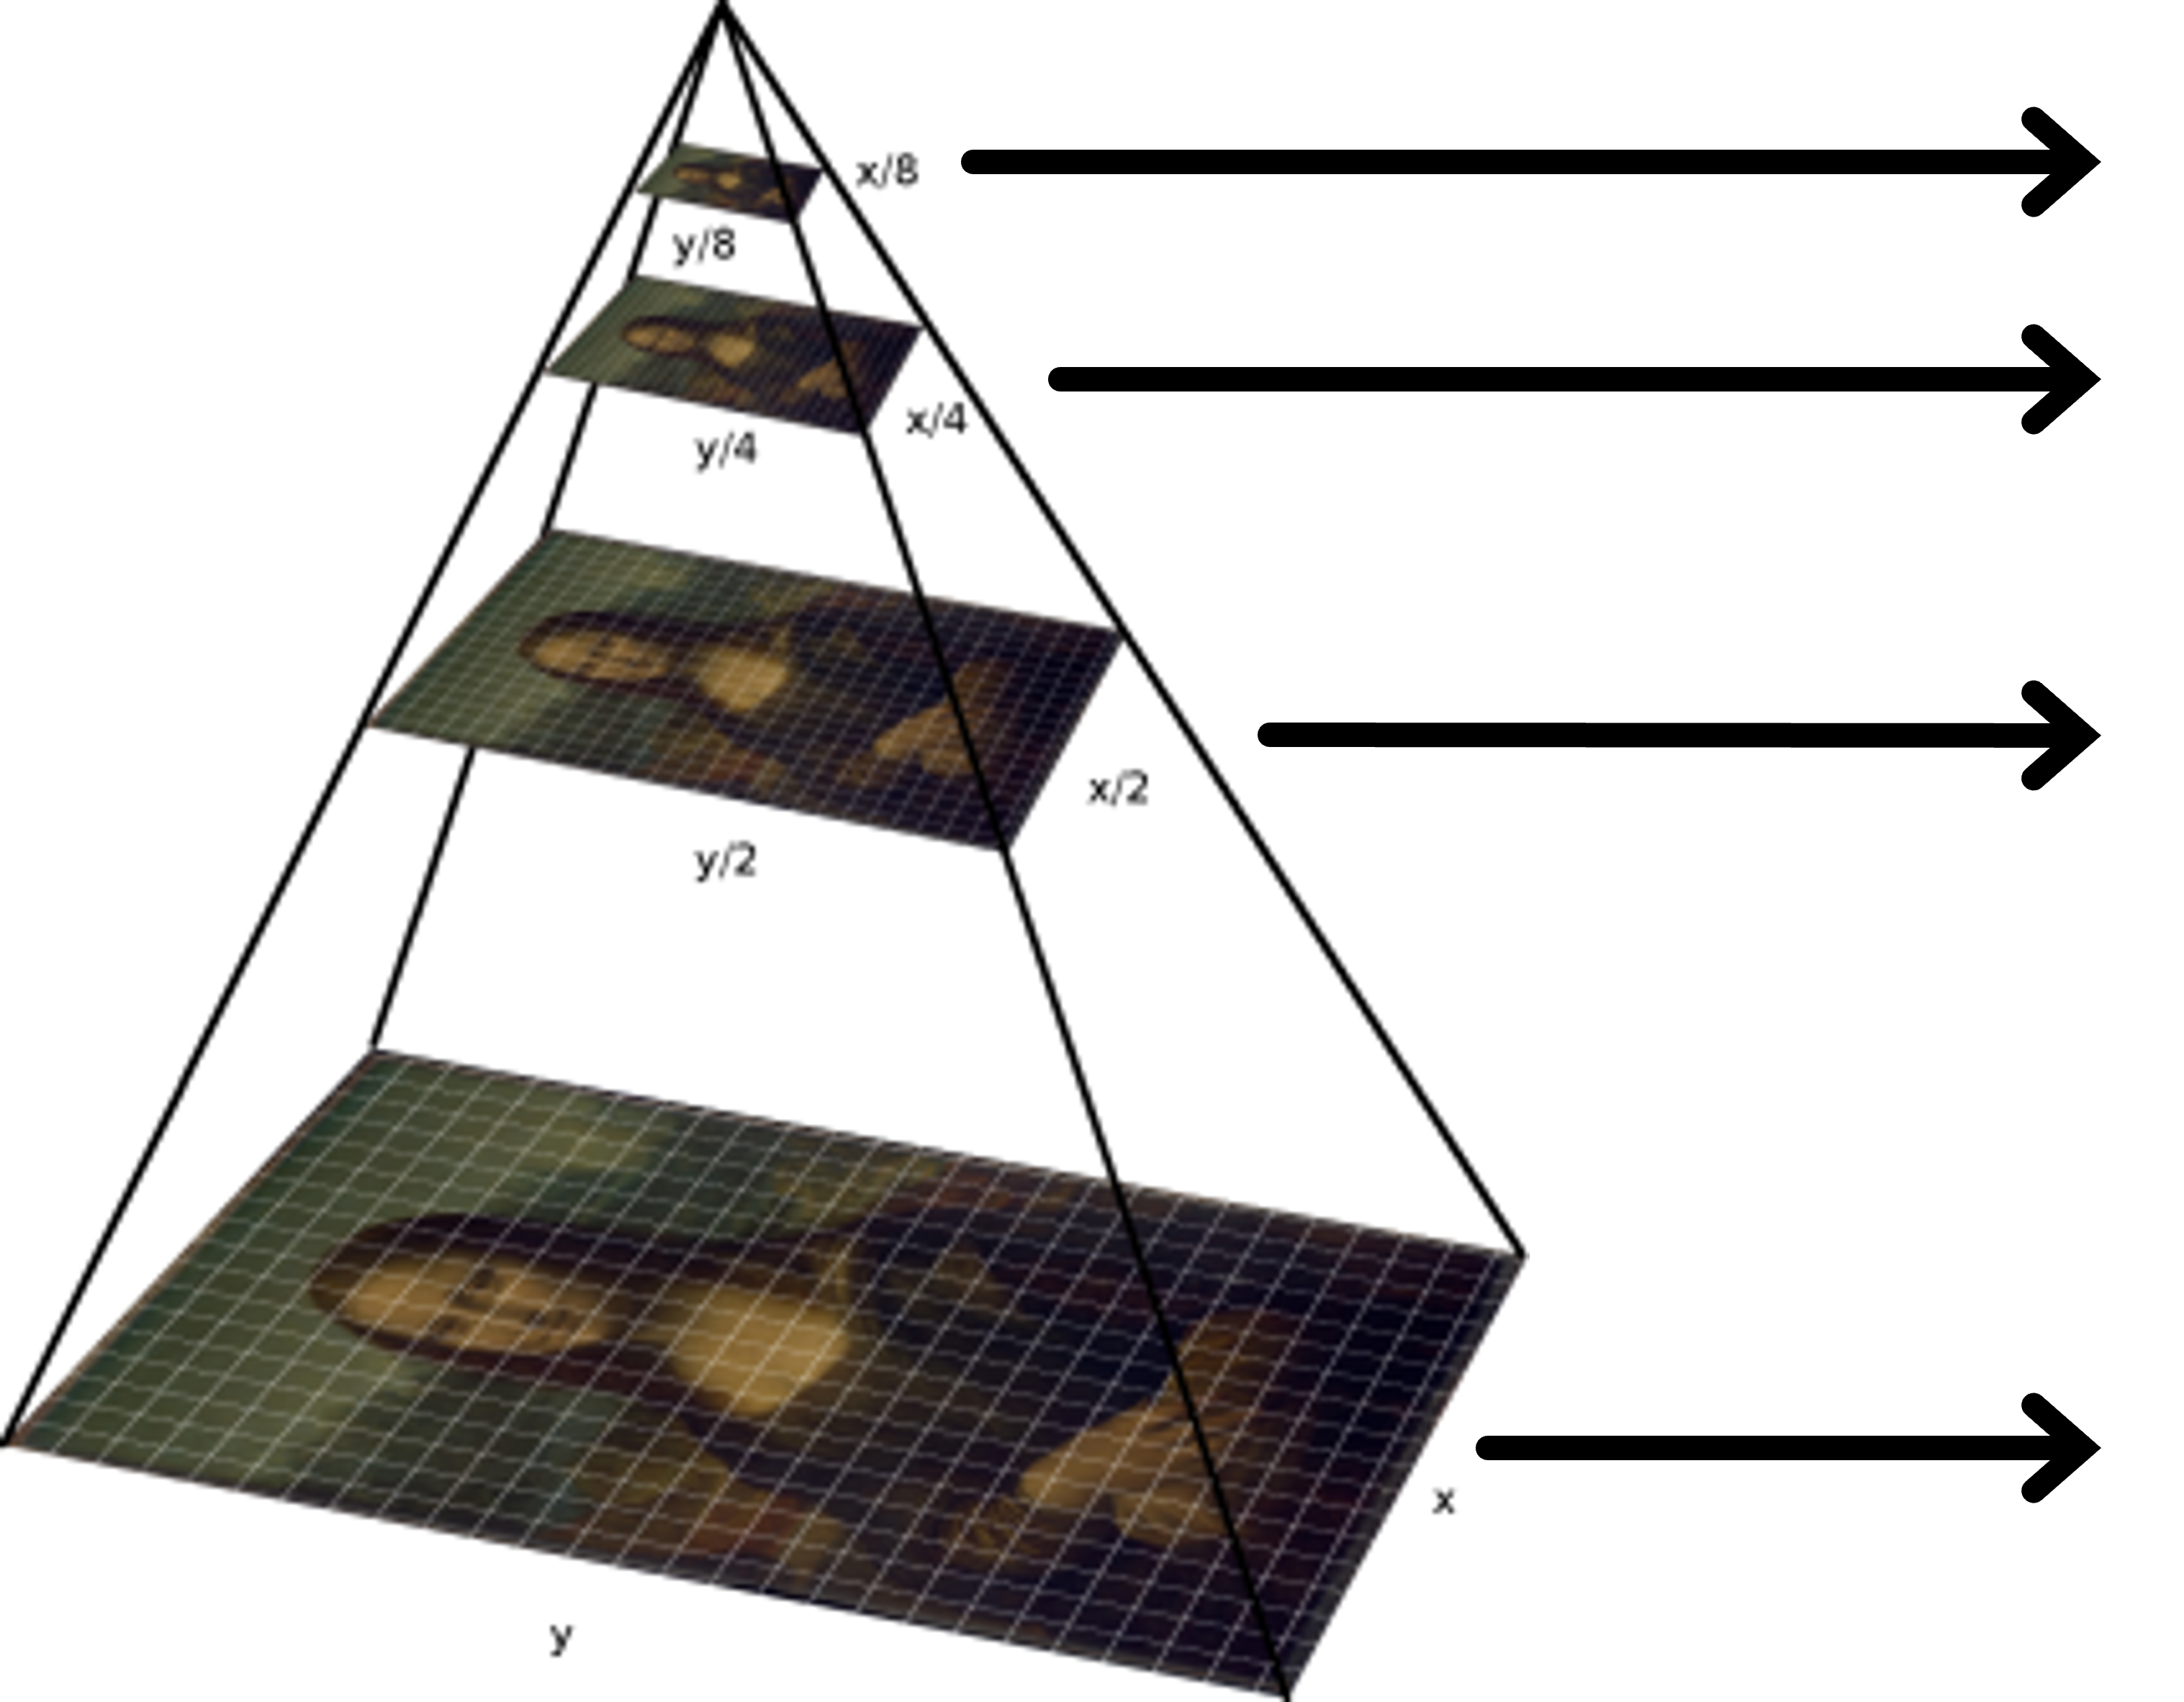
\includegraphics[width=0.5\linewidth]{orb_pyramid.png}
	\caption{\textit{Image Pyramid} pada ORB}
	\label{fig:orb_pyramid}	
\end{figure}

Tahap ini akan menghasilkan \textit{keypoint-keypoint} dengan skala yang berbeda sesuai dengan ukuran gambar di mana \textit{keypoint} tersebut ditemukan. \textit{Keypoint-keypoint} yang dihasilkan tersebut juga perlu untuk disaring dengan menggunakan \textit{Harris Corner Measure} seperti yang dijelaskan pada subbab sebelumnya. 

\subsection{Penentuan Orientasi}
\label{subsec:orb_orientasi}
Orientasi \textit{keypoint} pada ORB ditentukan oleh sudut antara sumbu $x$ dan vektor dari \textit{keypoint} menuju titik \textit{Intensity Centroid} dari daerah sekitarnya. \textit{Intensity Centroid} pada sebuah daerah gambar merupakan titik di mana terjadi perubahan nilai intensitas terbesar. Titik \textit{Intensity Centroid} ($C$) didefinisikan pada Persamaan~\ref{eq:centroid}.
\begin{equation}
	C=(\frac{m_{10}}{m_{00}}, \frac{m_{01}}{m_{00}})
	\label{eq:centroid}
\end{equation}
\textit{Centroid} ditentukan dengan menghitung \textit{moment} pada gambar yang didefinisikan pada Persamaan~\ref{eq:moment}.
\begin{equation}
	m_pq=\sum_{x,y}x^py^qI(x,y)
	\label{eq:moment}
\end{equation}
Pada Persamaan~\ref{eq:centroid} $m_{10}$ merupakan \textit{moments} gambar dari arah sumbu $x$. \textit{Moments} dari arah sumbu $x$ merupakan nilai perubahan intensitas yang dihitung dari sumbu tersebut, dihitung dari total seluruh nilai \textit{pixel} dikalikan dengan posisinya pada sumbu $x$. Sedangkan $m_{01}$ merupakan \textit{moments} dari arah sumbu $y$ yang dihitung dengan cara yang sama. Kedua nilai tersebut---$m_{10}$ dan $m_{01}$---masing-masing dibagi oleh $m_{00}$ yang didapat dengan menghitung jumlah dari nilai semua \textit{pixel} pada daerah yang diperiksa.

Titik \textit{centroid} dihitung pada daerah yang dikelilingi 16 \textit{pixel} yang digunakan pada tahap Penentuan \textit{Keypoint}. Dari daerah tersebut didapat titik yang merupakan \textit{centroid}. Lalu dibuat garis vektor yang berasal dari titik \textit{keypoint} (titik tengah) menuju titik \textit{centroid}. Orientasi ditentukan dari sudut antara garis lurus sumbu x dengan garis vektor.

Proses penentuan orientasi ini diilustrasikan pada Gambar~\ref{fig:orb_orientation}. Pada gambar tersebut titik dengan lingkaran hijau merupakan titik ditemukannya \textit{keypoint}. Penentuan orientasi dilakukan dengan mencari titik \textit{centroid} pada daerah yang dikelilingi lingkaran biru. Setelah didapat titik \textit{centroid} (lingkaran merah) maka orientasi merupakan garis lurus dan vektor dari titik \textit{keypoint} ke \textit{centroid}, ditunjukkan oleh $\theta$.
\begin{figure}[H]
	\centering
	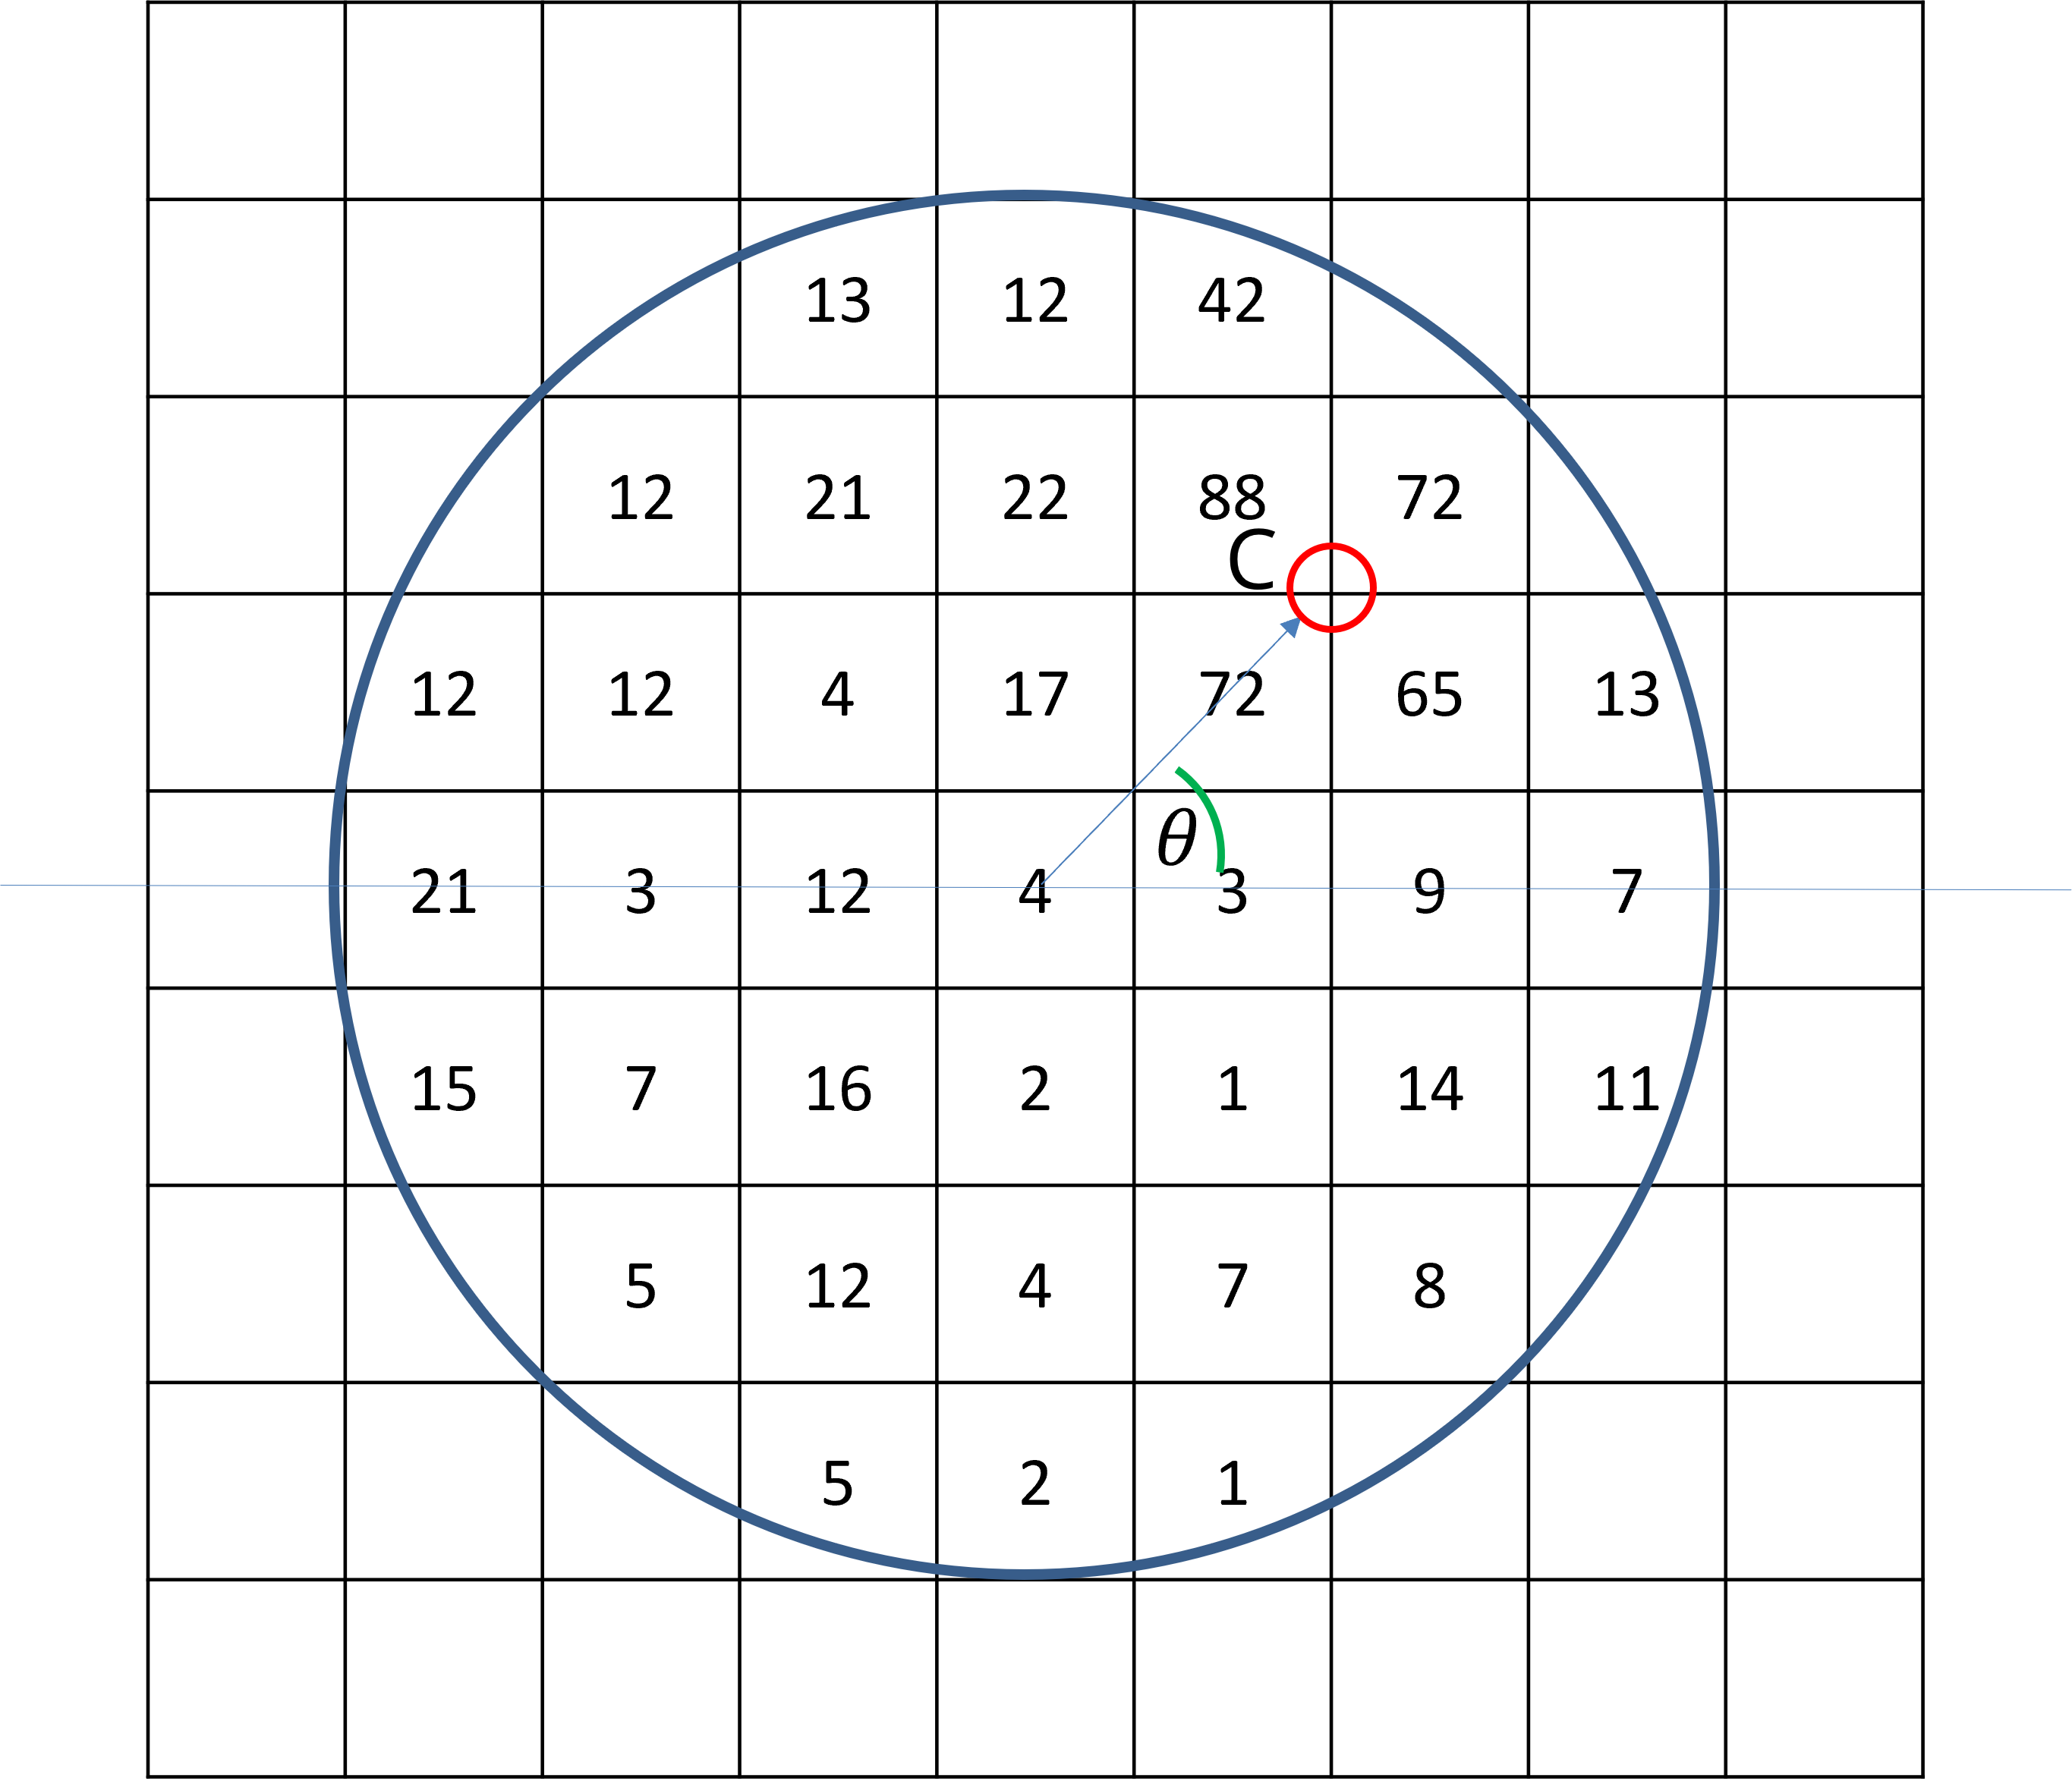
\includegraphics[scale=0.5]{orb_orientation.png}
	\caption{Ilustrasi penentuan orientasi pada ORB.}
	\label{fig:orb_orientation}
\end{figure}

\subsection{Pembuatan Deskriptor}
\label{subsec:orb_deskriptor}
Untuk setiap \textit{keypoint} yang dihasilkan perlu untuk dibuat sebuah vektor yang mendeskripsikan daerah di sekitar \textit{keypoint} tersebut. Vektor deskriptor berguna untuk melakukan identifikasi pada \textit{keypoint} tersebut. Pada ORB, vektor deskriptor berbentuk vektor biner berjumlah 256 elemen. Vektor didapat dengan melihat perbandingan nilai intensitas \textit{pixel} pada daerah di sekitar \textit{keypoint}.

Agar deskriptor bersifat invarian terhadap rotasi gambar terlebih dahulu dirotasi sesuai dengan orientasi yang sudah didapat sebelumnya. Dari gambar yang telah dirotasi diambil daerah berukuran $31\times31$ untuk dilakukan \textit{binary test}. \textit{Binary test} adalah fungsi yang membandingkan nilai intensitas antar dua titik pada gambar. Fungsi \textit{binary test} $\tau$ didefinisikan sebagai berikut:
\begin{equation}
	\tau(p;x,y)=\begin{cases}
		1 :p(x) < p(y), \\
		0 :p(x) \geq p(y)
	\end{cases}
\end{equation}
Fungsi tersebut akan menghasilkan nilai $1$ atau $0$ bergantung pada nilai intensitas dari dua titik yang dibandingkan.

Hasil dari \textit{binary test} yang dilakukan dengan membandingkan nilai dari pasangan-pasangan \textit{pixel} pada gambar akan sangat terpengaruh oleh \textit{noise} yang ada pada gambar. Jika pada saat melakukan \textit{binary test} digunakan \textit{pixel} yang merupakan \textit{noise} maka hasilnya akan tidak representatif terhadap sifat daerah sebenarnya. Untuk menangani masalah ini perlu terlebih dahulu dilakukan \textit{smoothing} pada gambar tersebut. ORB melakukan \textit{smoothing} dengan menggunakan \textit{integral image}. 

\textit{Integral image} adalah sebuah \textit{matrix} 2 dimensi yang dapat digunakan untuk menghitung hasil penjumlahan semua nilai \textit{pixel} di sebuah daerah pada gambar. \textit{Integral Image} dapat mempercepat proses penghitungan total nilai \textit{pixel} pada sebuah daerah dari gambar dengan ukuran berapapun. Nilai sebuah elemen pada koordinat $(x,y)$ di \textit{Integral Image} adalah total penjumlahan semua nilai yang posisi koordinatnya lebih kecil atau sama dengan $(x,y)$, seperti diilustrasikan pada Gambar~\ref{fig:integral_image1}.
\begin{figure}[H]
	\centering
	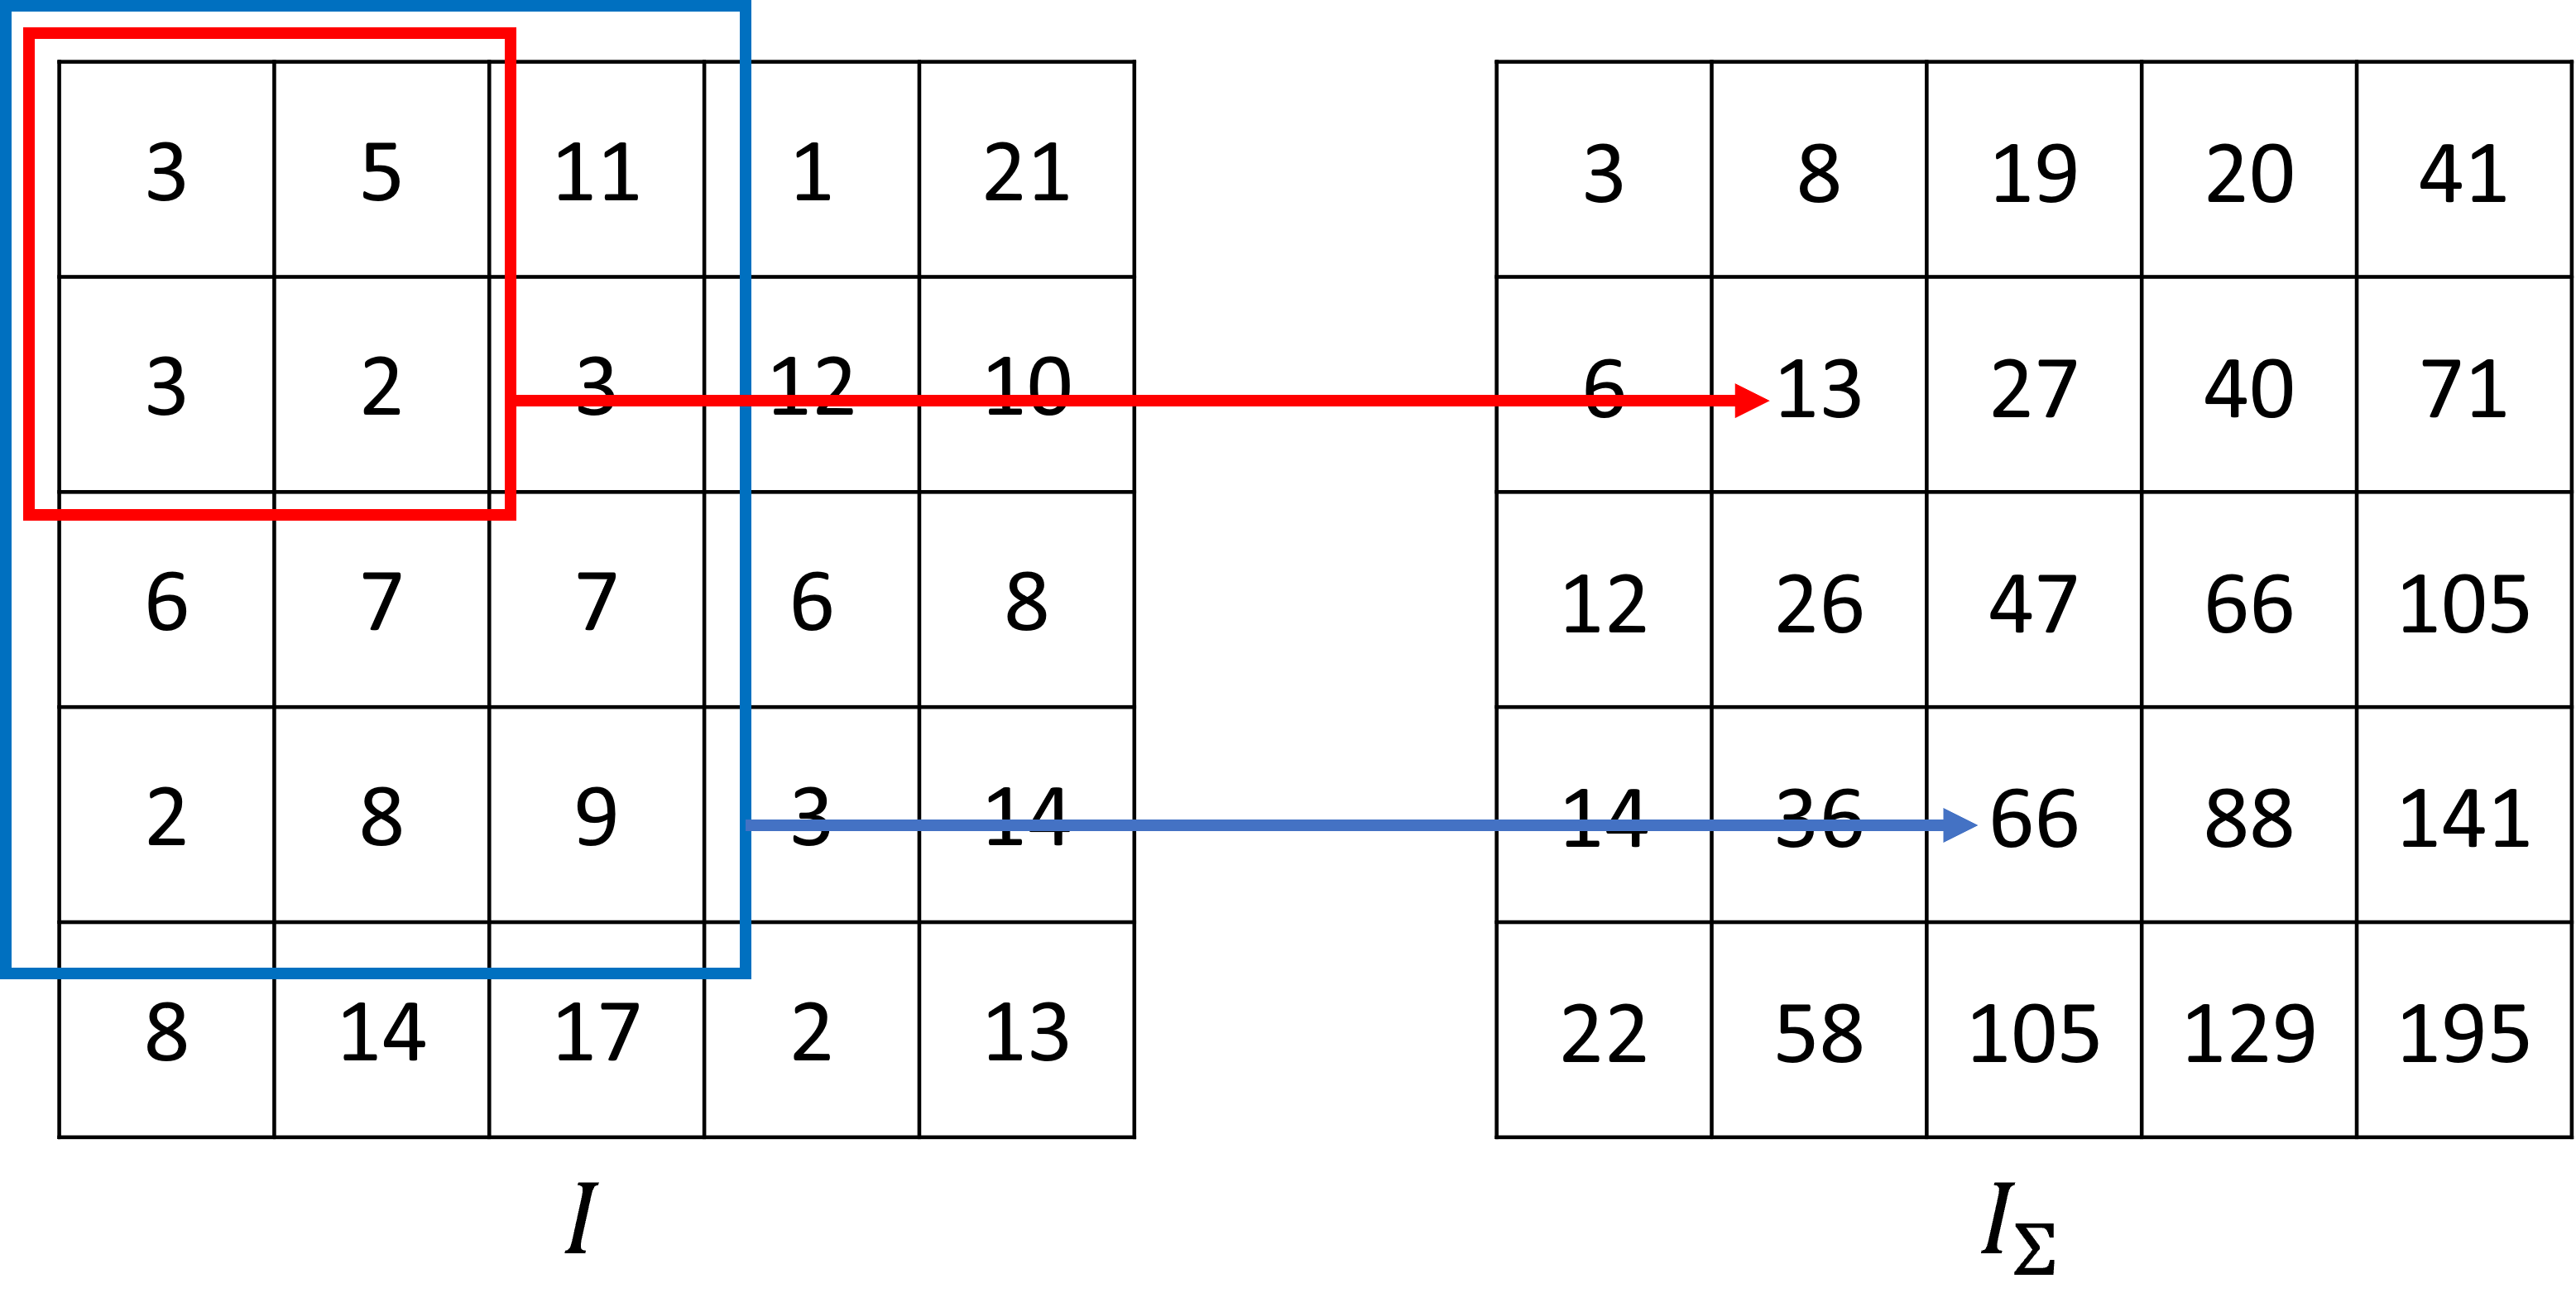
\includegraphics[scale=0.5]{ilustrasi_integral_image1.png}
	\caption{Ilustrasi penghitungan \textit{Integral Image}. \textit{Matrix} $I$ merupakan \textit{matrix} awal dan \textit{Matrix} $I_\Sigma$ merupakan \textit{Integral Image} dari $I$.}
	\label{fig:integral_image1}
\end{figure}

Gambar~\ref{fig:integral_image1} menunjukkan cara menghitung nilai elemen pada sebuah koordinat. Kotak pada \textit{Matrix} $I$ merupakan daerah yang dihitung total nilainya untuk mendapatkan nilai pada \textit{Matrix} $I_\Sigma$ yang ditunjuk oleh tanda panah. 

\textit{Matrix Integral Image} yang sudah dihasilkan dapat digunakan untuk menghitung nilai total dari sebuah daerah berukuran berapapun dengan melakukan operasi penjumlahan dan pengurangan pada 4 angka. Sebuah daerah pada Gambar I yang sudah dibuat \textit{Integral Image}-nya ($I_\Sigma$) yang berada pada persegi dengan titik pojok kiri atas $(T_x, T_y)$ dan pojok kanan bawah $(B_x, B_y)$ dapat dihitung nilai total elemennya dengan persamaan berikut:
\begin{equation}
	Su(T_x, T_y, B_x, B_y) = I_\Sigma(B_x, B_y) - I_\Sigma(B_x, T_y-1) - I_\Sigma(T_x-1, B_y) + I_\Sigma(T_x-1,T_y-1)
\end{equation}
Proses penghitungan nilai total sebuah daerah menggunakan \textit{Integral Image} diilustrasikan pada Gambar~\ref{fig:integral_image2}. Total nilai elemen dari daerah yang di dalam kotak biru pada Gambar $I$ dapat dihitung dengan menjumlahkan elemen pada Gambar $I_\Sigma$ yang diberi kotak hijau dan menguranginya dengan elemen yang diberi kotak merah. Daerah di dalam kotak biru tersebut memiliki nilai total $141-41-36+8=72$.
\begin{figure}[H]
	\centering
	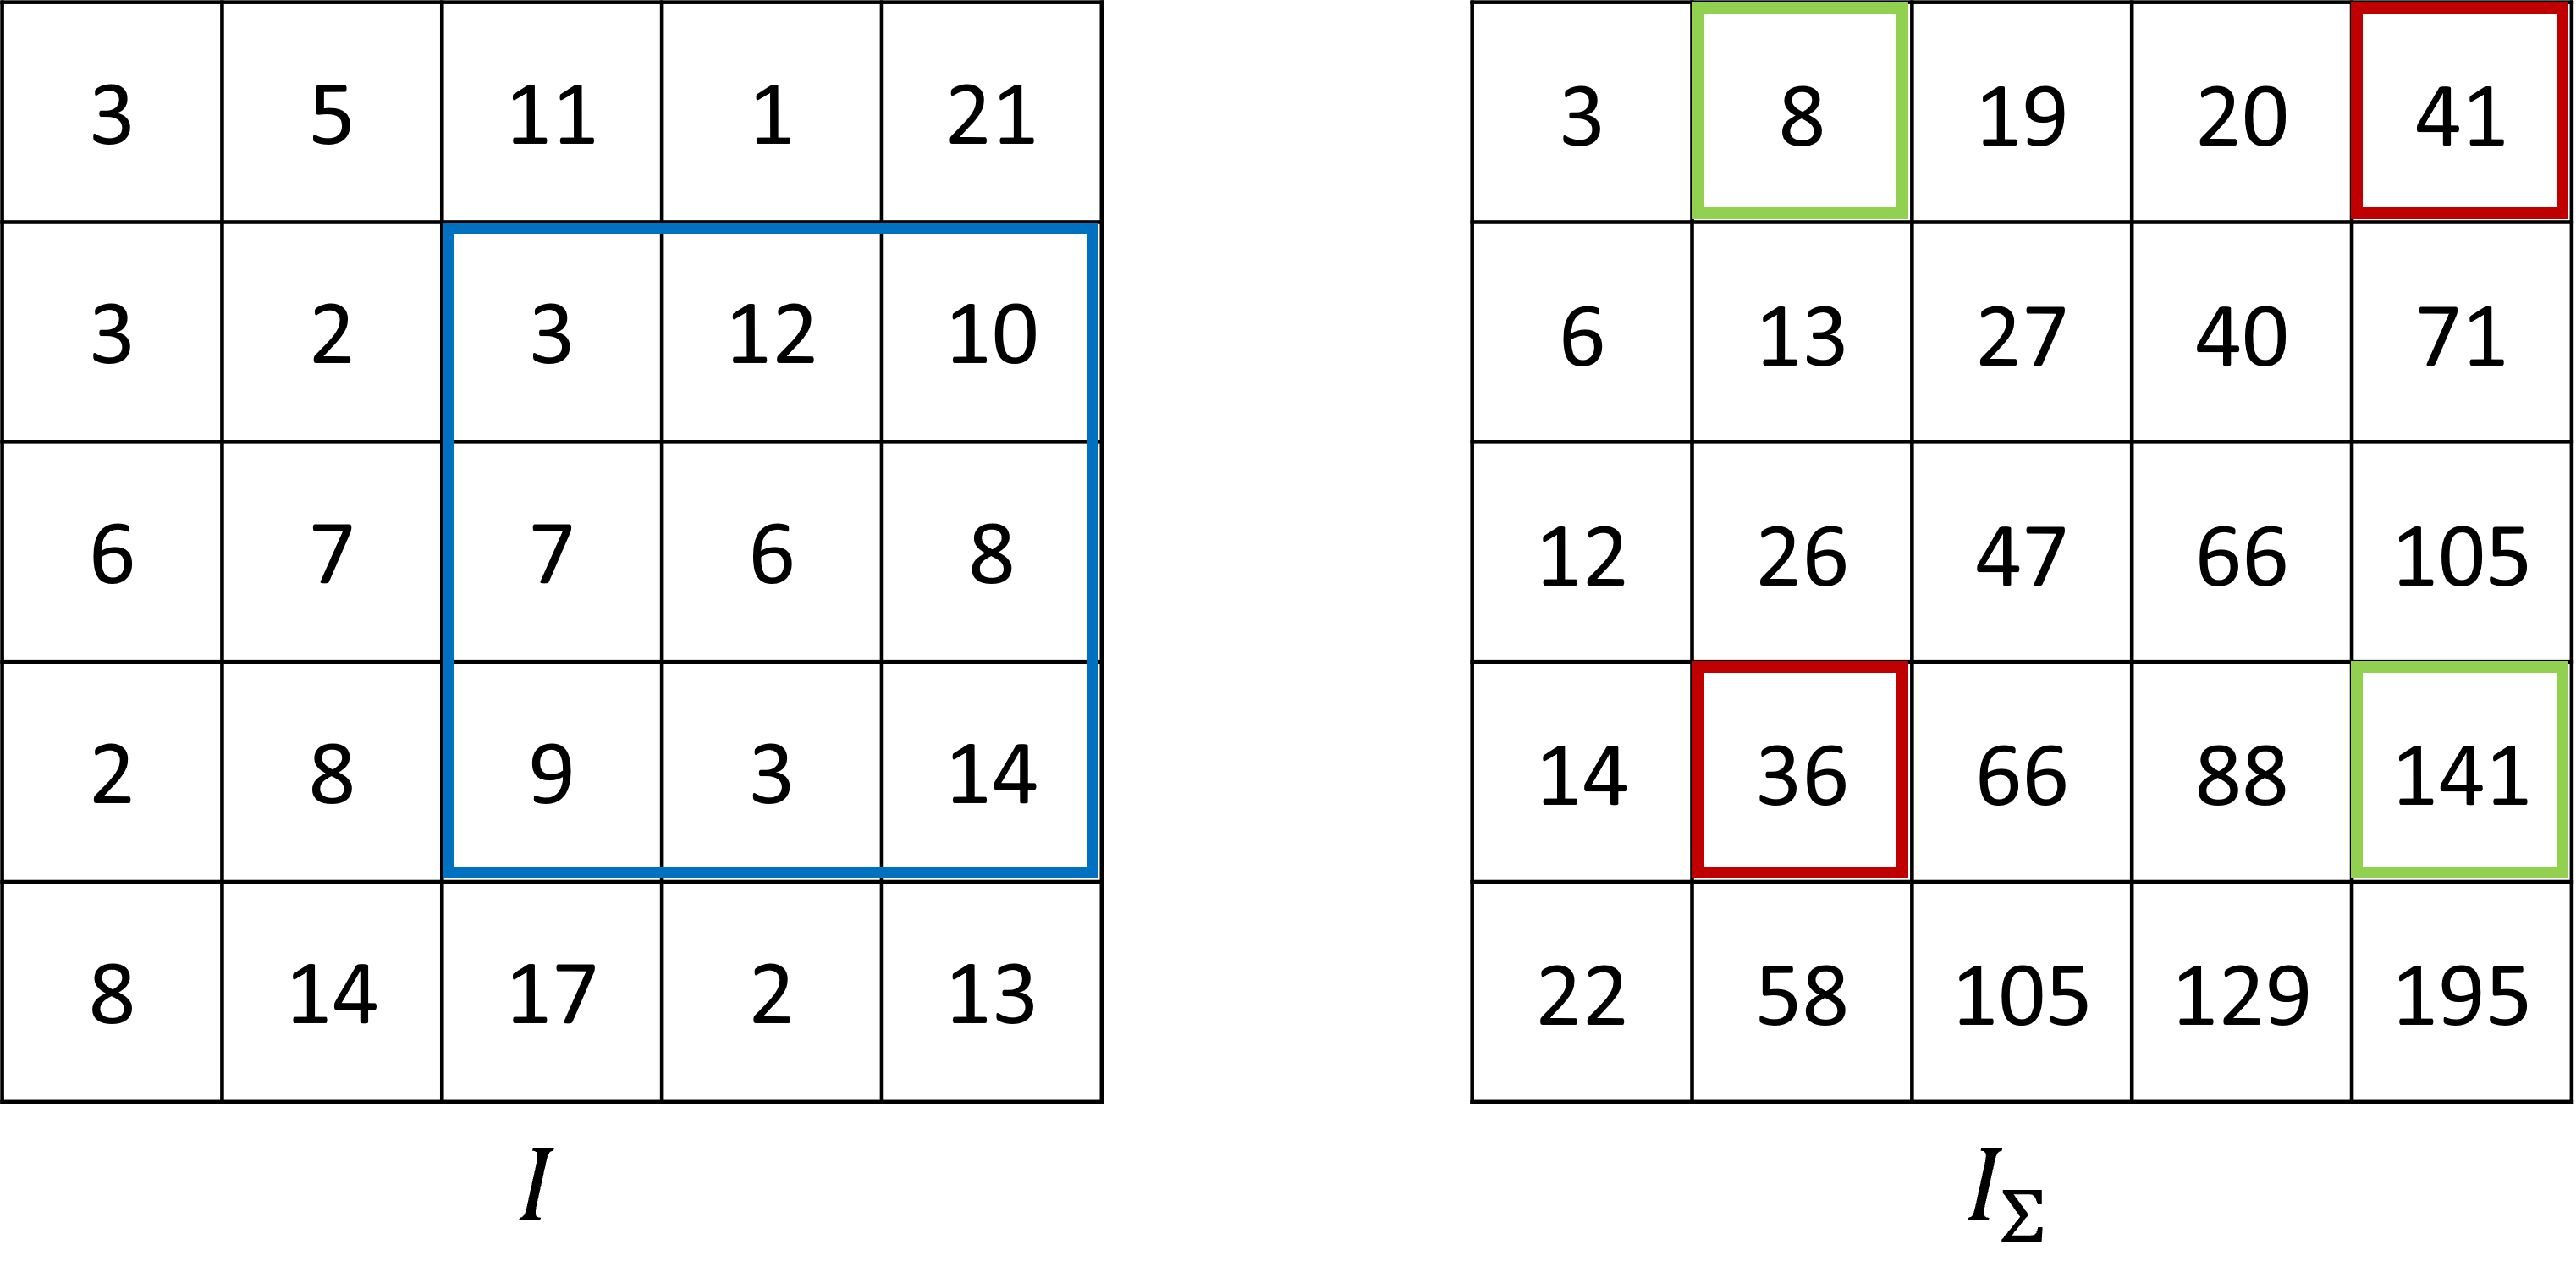
\includegraphics[scale=0.5]{ilustrasi_integral_image2.png}
	\caption{Penghitungan nilai total sebuah daerah dengan menggunakan \textit{Integral Image}}
	\label{fig:integral_image2}
\end{figure}

\textit{Smoothing} pada ORB dilakukan dengan mengubah \textit{binary test} yang dilakukan. \textit{Binary test} pada ORB dilakukan dengan membandingkan nilai total \textit{pixel} dari dua daerah berukuran $5\times5$ dalam daerah $31\times31$ yang digunakan untuk menghitung deskriptor. Penghitungan nilai total pada daerah $5\times5$ dilakukan dengan menggunakan \textit{Integral Image} untuk mempercepat proses. 

\textit{Binary test} pada ORB dilakukan sebanyak 256 kali untuk menghasilkan 256 elemen untuk vektor. ORB menggunakan 256 pasangan \textit{binary test} yang sudah ditentukan sebelumnya. Pasangan-pasangan tersebut didapat dari eksperimen yang dilakukan pada~\cite{rublee2011orb}.

\subsection{ORB di OpenCV}
\textit{Library} OpenCV di Python memiliki implementasi untuk metode ORB. Implementasi ORB ini memiliki kegunaan dan cara penggunaan yang mirip dengan implementasi SIFT. Untuk melakukan deteksi fitur lokal perlu untuk terlebih dahulu dibuat objek ORB dengan fungsi \texttt{ORB\_create}. Beberapa parameter fungsi \texttt{ORB\_create} yang relevan terhadap skripsi ini adalah:
\begin{itemize}
	\item \texttt{nfeatures}: jumlah maksimum fitur lokal yang dihasilkan.
	\item \texttt{scaleFactor}: rasio pengurangan resolusi pada setiap level \textit{pyramid}.
	\item \texttt{nlevels}: jumlah tingkatan (\textit{level}) pada \textit{pyramid}.
	\item \texttt{firstLevel}: tingkat dalam \textit{pyramid} sebagai tempat gambar asli.
	\item \texttt{patchSize}: ukuran daerah yang digunakan untuk membuat deskriptor.
\end{itemize}

Objek ORB tersebut lalu dapat digunakan untuk mendeteksi fitur lokal dalam gambar dengan menggunakan fungsi \texttt{detectAndCompute}.Fungsi \texttt{detectAndCompute} menerima beberapa parameter berikut:
\begin{itemize}
	\item \texttt{image}: gambar masukkan yang ingin dideteksi \textit{keypoint}-nya. Berbentuk \textit{array} 2 dimensi.
	\item \texttt{mask}: \textit{array} 2 dimensi dengan ukuran yang sama dengan gambar, menentukan \textit{pixel} mana yang digunakan dan yang tidak.
\end{itemize}

Fungsi tersebut menghasilkan \textit{tuple} berisi objek \textit{keypoint} dan array vektor deskriptor untuk tiap objek \textit{keypoint}. Setiap vektor merupakan vektor berisi bilangan biner berjumlah 256 elemen. Objek \textit{keypoint} memiliki atribut sebagai berikut:
\begin{itemize}
	\item \textbf{pt}: atribut ini memiliki dua buah atribut \textbf{x} dan \textbf{y} yang menunjukkan koordinat dari \textit{keypoint}.
	\item \textbf{size}: diameter daerah di sekitar \textit{keypoint} yang diperiksa.
	\item \textbf{angle}: orientasi dari \textit{keypoint}.
	\item \textbf{octave}: lapisan \textit{pyramid} di mana \textit{keypoint} tersebut didapatkan.
\end{itemize}

\section{BSIS (Best Score Increasing Subsequence)}
\label{sec:bsis}
Pada tahapan OIR (lihat~\ref{sec:oir}) sebuah pasangan fitur lokal perlu untuk memiliki sifat yang mirip (dilihat dari vektor deskriptornya) dan juga konsisten secara geometris. Pasangan yang konsisten secara geometris adalah pasangan yang memiliki posisi spasial yang konsisten terhadap pasangan lain di sekitarnya (contoh dapat dilihat pada Gambar~\ref{fig:geo_ver} di \ref{sec:oir}). BSIS~\cite{kusuma2019geometric} adalah salah satu metode yang dapat digunakan untuk menentukan apakah pasangan fitur lokal bersifat konsisten secara geometris. 

BSIS merupakan modifikasi metode WLIS~\cite{kusuma2012appearance} yang merupakan implementasi dari OIR. Modifikasi terdapat pada tahap \textit{Pairing}, \textit{Verification}, dan \textit{Scoring}. 

Tahapan dari BSIS dilakukan setelah fitur lokal telah diekstrak dari gambar \textit{query} dan gambar \textit{training} (gambar yang ada di \textit{dataset}). Tahapan BSIS ini dilakukan untuk setiap pemasangan gambar \textit{query} dan gambar \textit{training}. Pasangan gambar dengan skor tertinggi ditentukan sebagai pasangan yang benar dari gambar \textit{query}. Rincian tahapan dijabarkan pada subbab-subbab di bawah ini. 

\subsection{Pairing}
\label{subsec:bsis_pairing}
Pada tahap awal setiap fitur lokal pada gambar \textit{query} akan dicari $N$ fitur lokal dari gambar \textit{training} yang nilai kemiripan vektor deskriptornya paling tinggi. Pencarian $N$ pasangan paling mirip dilakukan dengan menggunakan KD-Tree (lihat~\ref{sec:kdtree}) untuk mempercepat waktu komputasi. Pasangan-pasangan ini akan memiliki sebuah skor kemiripan yang dihitung dari vektor deskriptor kedua fitur lokal. Tidak semua dari $N$ pasangan paling mirip akan digunakan dalam proses BSIS. 

Untuk setiap fitur lokal, BSIS hanya akan mengambil beberapa pasangan yang benar-benar mirip atau paling berpeluang menjadi pasangan yang benar. Pasangan yang benar-benar mirip pada BSIS adalah pasangan yang nilai kemiripannya tinggi dan memiliki perbedaan yang cukup jauh dengan nilai kemiripan pasangan lain. 

BSIS menganggap pasangan-pasangan yang sangat mirip adalah pasangan yang nilai kemiripannya tinggi dan merupakan \textit{outlier}. Penentuan \textit{outlier} dilakukan dengan menggunakan \textit{mean} dan deviasi standar. Penggunaan \textit{mean} dan deviasi standar untuk menentukan \textit{outlier} karena BSIS mengasumsikan bahwa nilai kemiripan pasangan-pasangan dari sebuah fitur lokal terdistribusi secara normal. 

BSIS menentukan \textit{outlier} seperti pada Persamaan~\ref{eq:outlier}. Untuk sebuah fitur lokal gambar \textit{training} $P_Q$ yang dipasangkan dengan gambar \textit{training} $P_T$, pasangan tersebut hanya akan digunakan jika nilai kemiripannya lebih dari \textit{mean} $(m)$ ditambah konstanta $K$ dikali deviasi standar $(\sigma)$. \textit{Mean} merupakan rata-rata dari nilai kemiripan dari $N$ pasangan $P_Q$ dan $\sigma$ merupakan nilai deviasi standarnya sedangkan untuk konstanta digunakan nilai $K=4$.

\vspace{-10px}
\begin{equation}
	\label{eq:outlier}
	similarity(P_Q, P_T) > m + (K \times \sigma)
\end{equation}

Pasangan-pasangan yang telah dipilih (merupakan \textit{outlier}) tersebut lalu diberi bobot berdasarkan nilai kemiripannya. Bobot sebuah pasangan didapatkan dengan menghitung seberapa jauh nilai kemiripan pasangan tersebut terhadap rata-rata dengan memperhatikan penyebaran nilainya. Bobot $(P_w)$ untuk sebuah pasangan dari fitur lokal $P_Q$ dan $P_T$ didefinisikan pada Persamaan~\ref{eq:pair_weight}.

\vspace{-7px}
\begin{equation}
	\label{eq:pair_weight}
	P_w(P_Q, P_T)=(\frac{similarity(P_Q, P_T) - m}{\sigma})^2
\end{equation}

$P_Q$ merupakan fitur lokal gambar \textit{query} dan $P_T$ merupakan fitur lokal dari gambar \textit{training}. Nilai $P_w$ yang semakin tinggi menunjukkan bahwa pasangan tersebut semakin berpotensi untuk menjadi pasangan yang tepat.

\subsection{Verification}
Pada tahap \textit{Pairing} telah didapat beberapa pasangan antara fitur lokal gambar \textit{query} dan gambar \textit{training} yang paling berpotensi merupakan pasangan yang benar. Dari tahap sebelumnya setiap fitur lokal pada gambar \textit{query} dapat dipasangkan dengan lebih dari 1 fitur lokal pada gambar \textit{training}. Pasangan-pasangan tersebut akan diperiksa pada tahap ini untuk mencari pasangan mana saja yang konsisten secara geometris. Setiap fitur lokal baik dari gambar \textit{query} maupun \textit{training} hanya akan berada dalam satu pasangan setelah dilakukan verifikasi.

Pasangan yang konsisten secara geometris adalah pasangan-pasangan yang memiliki posisi spasial yang konsisten terhadap pasangan fitur lokal lain di sekitarnya. Sifat konsisten ini ditunjukkan oleh posisi fitur-fitur lokal pada gambar \textit{query} dan gambar \textit{training}. Sebagai contoh, dua buah fitur lokal dari gambar \textit{query} $PQ_1$ dan $PQ_2$ dipasangkan dengan fitur lokal $PT_1$ dan $PT_2$ dari gambar \textit{training}. Jika $PQ_1$ berada di sebelah kiri $PQ_2$ ($PQ_1$ muncul lebih dulu dalam proyeksi sumbu $x$) maka $PT_1$ juga harus berada di sebelah kiri $PT_2$ untuk agar kedua pasangan tersebut dikatakan konsisten secara geometris.

Tahap \textit{Verification} pada BSIS bertujuan untuk menemukan pasangan-pasangan fitur lokal yang konsisten secara geometris sesuai dengan penjelasan di atas. BSIS melakukan verifikasi dengan memproyeksikan seluruh fitur lokal dari gambar \textit{query} dan \textit{training} pada sumbu $x$ dan mencari pasangan yang konsisten dan memiliki skor yang paling tinggi. Langkah-langkah verifikasi pada BSIS secara rinci adalah sebagai berikut:
\begin{enumerate}
	\item Ambil semua fitur lokal dari gambar \textit{query} dan proyeksikan pada sumbu $x$. Setiap fitur lokal akan diberi sebuah \textit{order} sesuai dengan urutan kemunculannya.
	\item Ambil semua fitur lokal dari gambar \textit{training} dan proyeksikan pada sumbu $x$. Urutkan fitur lokal tersebut sesuai dengan urutan kemunculannya.
	\item Buat tabel untuk fitur lokal pada dari gambar \textit{training} dengan setiap kolom merupakan fitur lokal yang diurutkan berdasarkan kemunculannya pada sumbu $x$;   
	\item Isi setiap kolom dengan pasangan-pasangan fitur lokal yang melibatkan fitur lokal kolom tersebut. Untuk tiap isi kolom, catat nomor \textit{order} dari fitur lokal gambar \textit{query} pasangan tersebut dan bobot $(P_w)$ pasangan tersebut. Kolom pada tabel merupakan fitur lokal pada gambar \textit{training} dan tiap barisnya merupakan fitur lokal pada gambar \textit{query}.
	\begin{figure}[H]
		\centering
		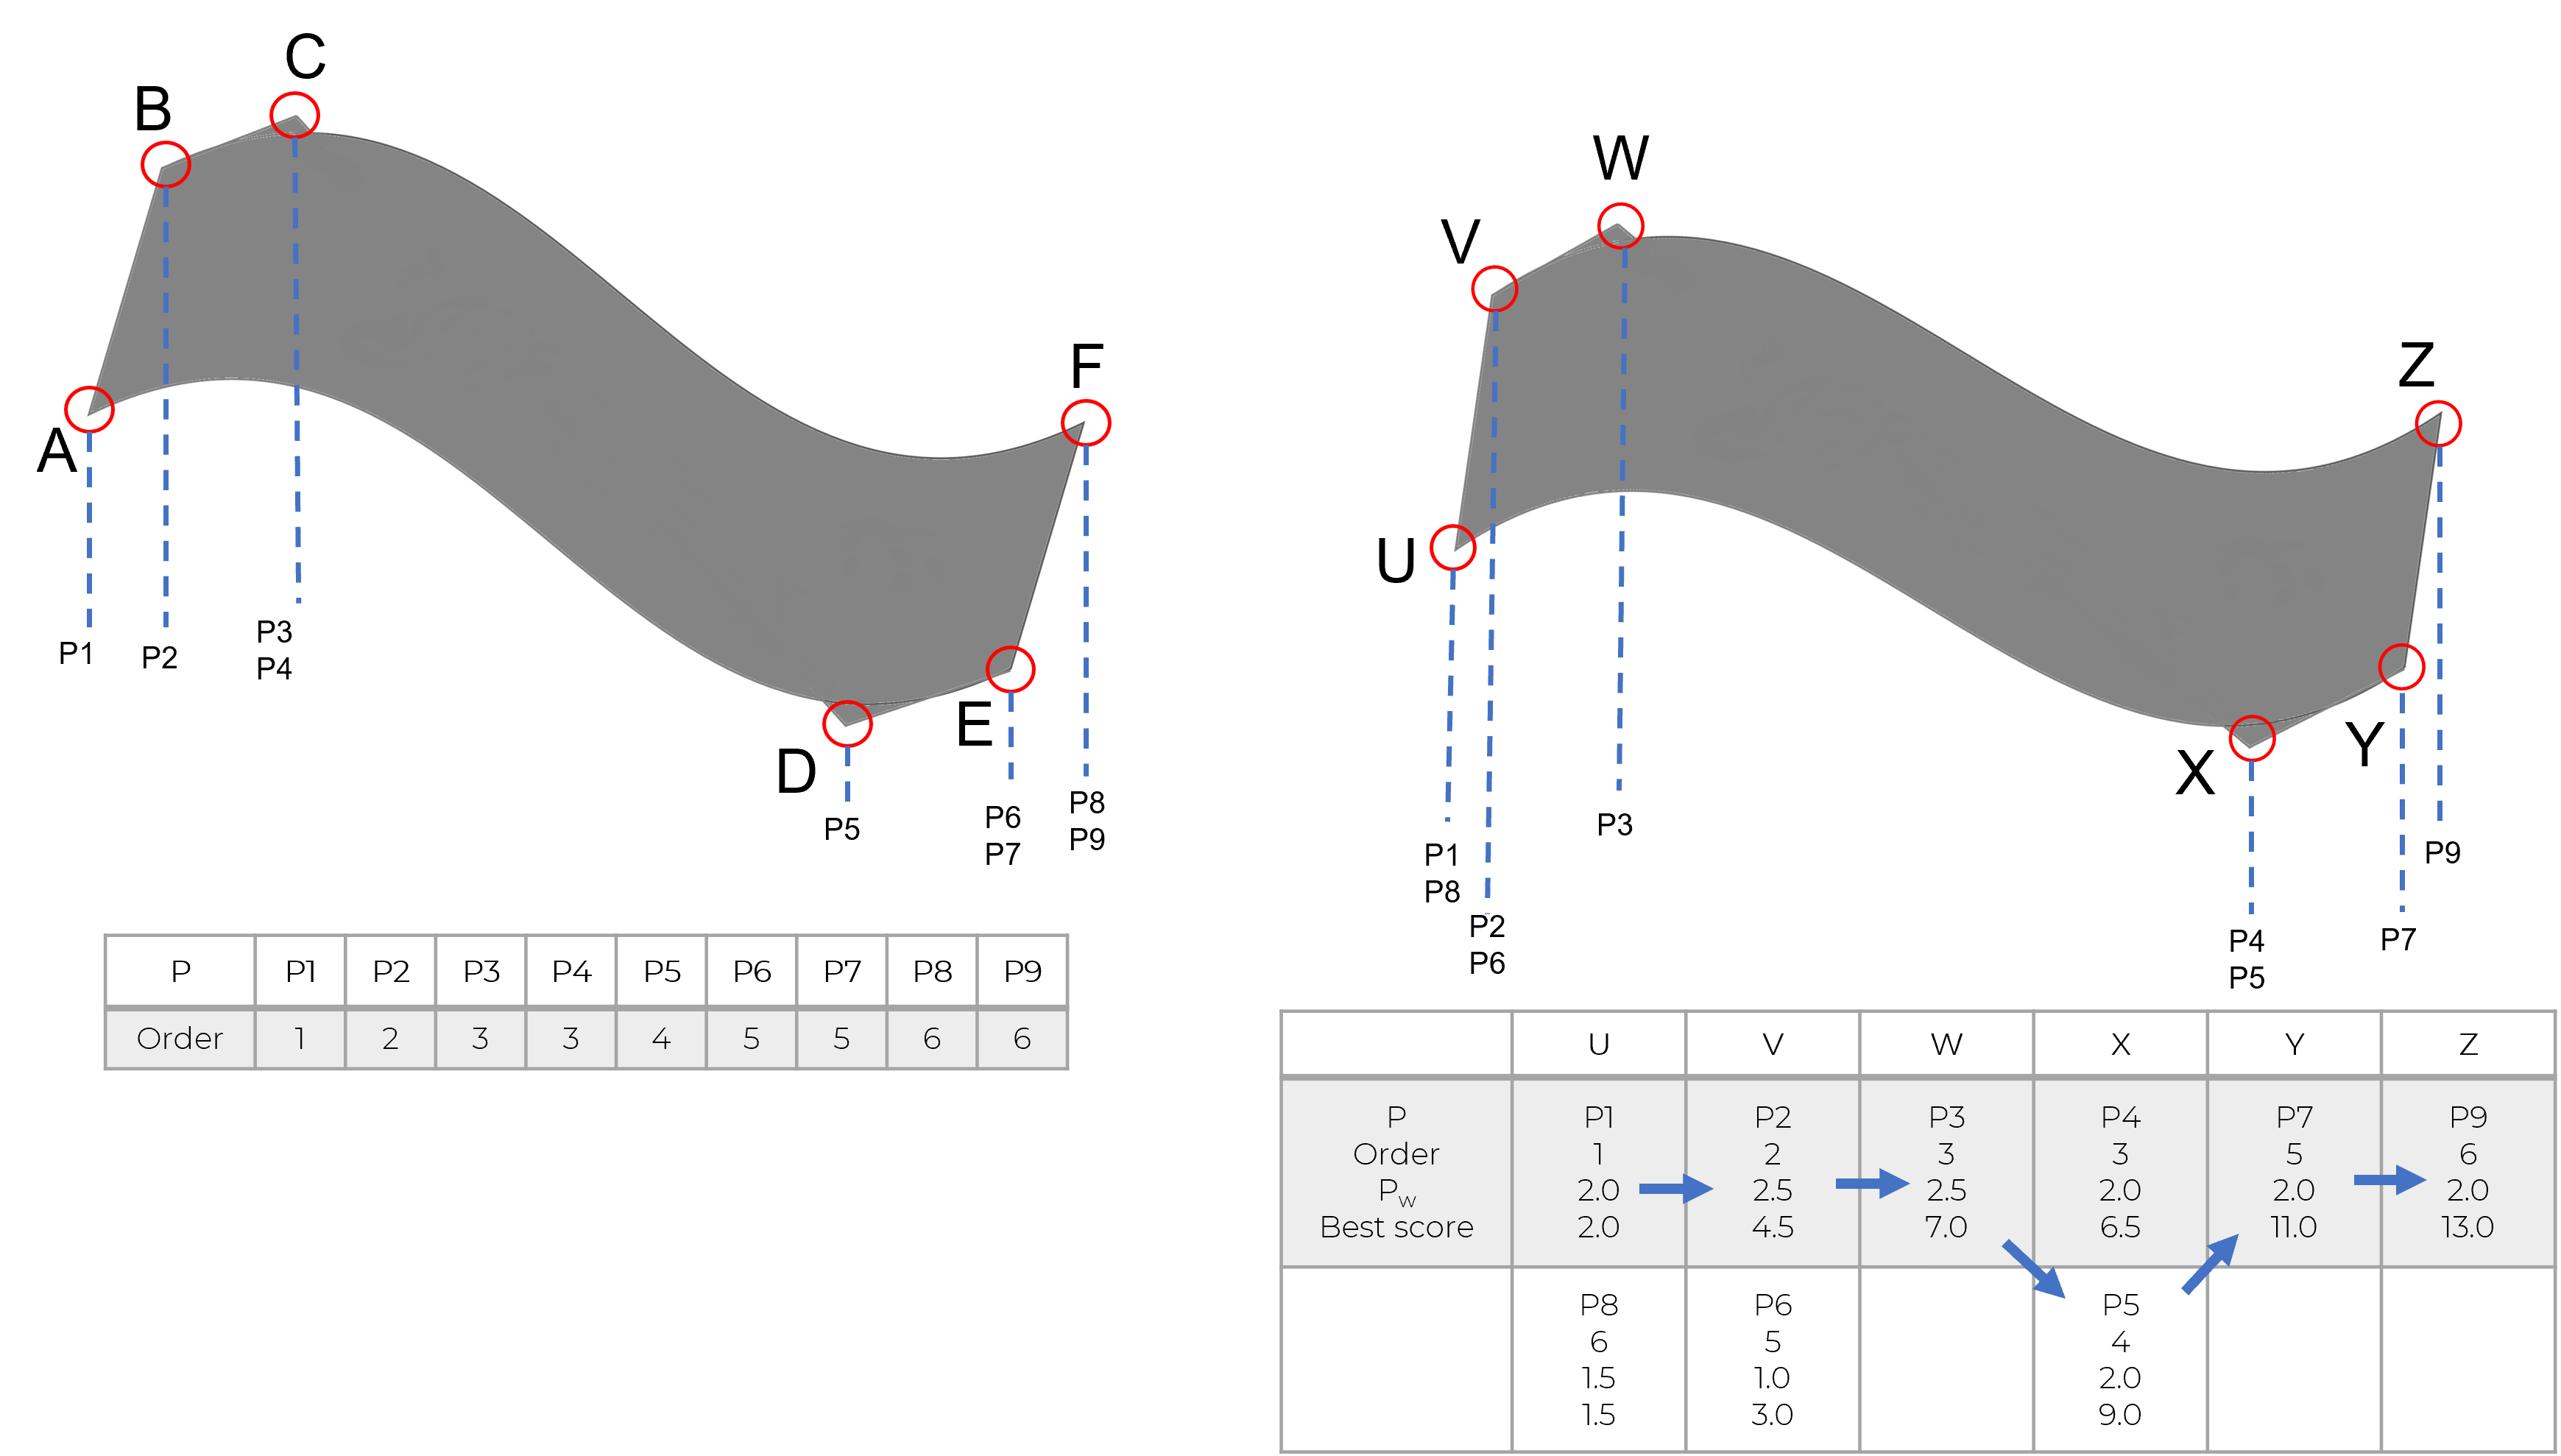
\includegraphics[scale=0.6]{bsis_verifikasi.png}
		\label{fig:bsis_verifikasi}
		\caption{Tahapan verifikasi pada BSIS.}
	\end{figure}
	\item BSIS hanya mengambil satu pasangan dari setiap fitur lokal di gambar \textit{query} dengan bobot pasangan yang tertinggi. Untuk itu buat sebuah \textit{subsequence} dengan mengambil satu baris dari tiap kolom berurutan mulai dari kolom paling kiri. \textit{Order} menunjukkan urutan kemunculan pasangan tersebut pada gambar \textit{query}, untuk itu \textit{order} dari \textit{subsequence} perlu untuk terus bertambah tiap elemen. \textit{Subsequence} yang dicari adalah yang memiliki total nilai bobot pasangan paling banyak.
	\item Verifikasi juga perlu dilakukan untuk sumbu $y$. Fitur lokal yang telah dipilih pada langkah sebelumnya (fitur lokal yang masuk dalam \textit{subsequence}) akan dilakukan verifikasi ulang menggunakan urutannya pada sumbu $y$.
\end{enumerate}
Tahapan di atas dilakukan beberapa kali pada untuk orientasi fitur lokal gambar \textit{training} yang berbeda untuk mencari orientasi gambar yang memberikan total skor pasangan paling tinggi.

\subsection{Scoring}
\label{subsec:bsis_scoring}
Setelah dipilih dan didapat pasangan fitur lokal yang konsisten secara geometris akan dihitung nilai kemiripan gambar masukkan dengan gambar \textit{training} yang terpilih. Tingkat kemiripan ditentukan dengan menghitung total $P_w$ dari pasangan yang terpilih pada tahap \textit{Verification}. Nilai kemiripan ini dapat digunakan untuk menentukan apakah pasangan gambar cukup mirip untuk menjadi pasangan yang benar.

\section{KD-Tree}
\label{sec:kdtree}
KD-Tree~\cite{bentley1975multidimensional} merupakan sebuah struktur data yang dapat digunakan untuk mencari vektor yang paling mirip dengan waktu proses yang relatif lebih singkat. Struktur KD-Tree digunakan untuk mencari sejumlah pasangan fitur lokal yang sifatnya paling mirip pada tahapan \textit{Pairing} di BSIS~\ref{sec:bsis}. 

Secara umum KD-Tree merupakan sebuah pohon pencarian biner di mana setiap \textit{node}-nya merupakan sebuah vektor berjumlah $k$-elemen. Setiap \textit{level} pada pohon membandingkan elemen vektor yang berbeda. \textit{Level} pertama pohon akan menggunakan elemen pertama dari vektor sebagai pembanding, elemen kedua pada \textit{level} kedua dan seterusnya. Saat \textit{level} dari pohon sudah mencapai $k - 1$, maka akan kembali ke elemen pertama. Elemen yang diperiksa pada \textit{level} $l$ di KD-Tree dengan jumlah $k$ elemen didefinisikan pada Persamaan~\ref{eq:target_kd-tree}.
\vspace{-4px}
\begin{equation}
	\label{eq:target_kd-tree}
	target(l, k) = l\bmod k
\end{equation}
Gambar~\ref{fig:kd-tree} menunjukkan contoh pohon KD-Tree dengan jumlah 3 elemen.
\begin{figure}[H]
	\centering
	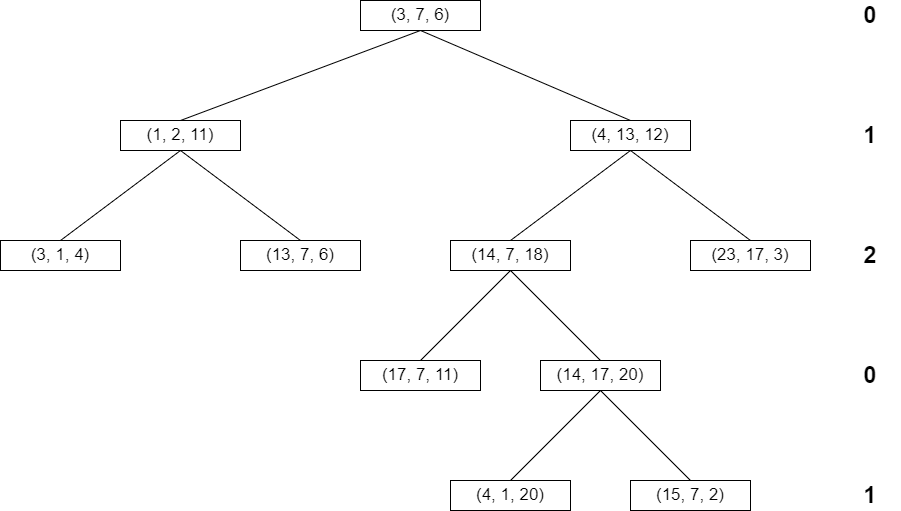
\includegraphics[scale=0.4]{kd-tree.png}
	\caption{Contoh pohon struktur KD-Tree. Angka di sebelah kanan menunjukkan elemen vektor yang diperiksa pada level tersebut.}
	\label{fig:kd-tree}
\end{figure}

KD-Tree membuat pohon dari sekumpulan vektor di \textit{dataset}. Vektor pertama yang masuk akan menjadi \textit{root} dari pohon. Vektor selanjutnya akan dibandingkan nilai elemen pertamanya dengan elemen pertama dari \textit{root}, jika nilainya lebih kecil maka vektor tersebut akan menjadi \textit{child} sebelah kiri dan menjadi \textit{child} sebelah kanan jika sebaliknya. Proses berlanjut untuk vektor selanjutnya, elemen di vektor yang masuk akan dibandingkan dengan vektor pada \textit{node} pohon sesuai dengan \textit{level} pohon saat itu. 

Setelah terbentuk pohon dari semua vektor pada \textit{dataset}, pohon tersebut dapat digunakan untuk pencarian tetangga terdekat (\textit{nearest neighbor search}) dari sebuah vektor masukkan baru. Tahapan untuk mencari tetangga terdekat dari vektor $Q$ pada sebuah pohon KD-Tree $K$ adalah sebagai berikut:
\begin{enumerate}
	\item Jelajahi pohon $K$ seperti biasa, dimulai dari \textit{node} \textit{root}. Bandingkan elemen pada \textit{node} tersebut dengan elemen pada $Q$. 
	\item Untuk semua \textit{node} yang diperiksa hitung jaraknya ke $Q$. Simpan jarak tersebut ke dalam variabel $closest$. Jika pada \textit{node} selanjutnya didapat jarak yang lebih kecil maka ganti $closest$ dengan jarak tersebut.
	\item Jelajahi sampai sudah mencapai \textit{node} yang merupakan \textit{leaf}. Pada titik ini masih mungkin ada \textit{node} pada bagian pohon yang tidak dijelajahi yang jaraknya lebih kecil dari $closest$.
	\item Untuk semua \textit{node} bukan \textit{leaf} yang dilewati hitung jarak elemen ke-$n$ dari $Q$ ke elemen ke-$n$ \textit{node} tersebut. Jika jaraknya lebih kecil dari $closest$ maka jelajahi \textit{child} dari \textit{node} tersebut yang sebelumnya tidak dipilih.
\end{enumerate}

\section{Clustering}
\label{sec:clustering}
\textit{Clustering} adalah salah satu teknik pengolahan data dalam \textit{machine learning}. Pada dasarnya \textit{clustering} akan membagi objek-objek pada \textit{dataset}  menjadi beberapa kelompok (\textit{cluster}) berdasarkan sifatnya. Objek-objek yang memiliki sifat mirip akan masuk kedalam satu kelompok. Sebuah pembagian \textit{cluster} yang baik adalah di mana setiap objek dalam \textit{cluster} memiliki sifat yang mirip dan antar \textit{cluster} memiliki sifat yang sangat berbeda.

Beberapa contoh metode \textit{clustering} yang ada adalah \textit{Agglomerative Clustering} dan DBSCAN. Kedua teknik tersebut menggunakan metode dasar yang berbeda dan akan menghasilkan \textit{cluster} dengan ciri yang berbeda juga. Kedua metode tersebut dijelaskan pada dua subbab berikut. Penjelasan berdasarkan pada~\cite{han2011data}

\subsection{Agglomerative Clustering}
\label{subsec:clustering_agglomerative}
Teknik \textit{Agglomerative Clustering} adalah salah satu teknik \textit{clustering} yang berbasis hierarki (\textit{hierarchical}). Teknik ini membentuk \textit{cluster} dengan menyusun hierarki atau tingkatan antar objek berdasarkan kemiripannya. Pasangan objek dengan jarak yang paling kecil akan berada di tingkatan terendah, jarak terkecil selanjutnya akan berada di tingkat atasnya, dan seterusnya hingga semua objek telah tercakup. 

\textit{Agglomerative Clustering} adalah teknik \textit{clustering} berbasis hierarki yang menggunakan metode \textit{bottom-up}. Metode \textit{bottom-up} memulai tahapan dengan membentuk \textit{cluster-cluster} kecil dan kemudian menggabungkan \textit{cluster} kecil tersebut menjadi \textit{cluster} yang lebih besar.

Tahapan \textit{Agglomerative Clustering} dimulai dengan terlebih dahulu menghitung jarak antar tiap objek. Setelah itu ambil pasangan dengan jarak paling kecil dan gabungkan menjadi satu \textit{cluster} dan lakukan juga untuk jarak paling kecil berikutnya. Jika jarak terkecil yang ada adalah antara objek yang sudah berada di dalam \textit{cluster}, maka gabungkan kedua \textit{cluster} tersebut menjadi \textit{cluster} yang lebih besar. 

Langkah-langkah pada tahapan tersebut dilakukan hingga semua objek sudah berada di dalam satu \textit{cluster} yang sama. \textit{Cluster} besar tersebut lalu dapat dibagi berdasarkan dari jaraknya dengan menggunakan \textit{threshold} yang dapat ditentukan secara manual.

Algoritma \textit{clustering Agglomerative} dapat dibagi menjadi beberapa tipe dibedakan dari cara menghitung jarak antar \textit{cluster-cluster}-nya. Teknik \textit{single-linkage} menghitung jarak antar \textit{cluster} dengan jarak objek terdekat antar kedua \textit{cluster} tersebut. Sedangkan teknik \textit{complete-linkage} menghitung jarak dengan jarak objek terjauh antar dua \textit{cluster}.

Proses penggabungan objek menjadi \textit{cluster} pada \textit{Agglomerative Clustering} ditunjukkan pada \textit{Pseudocode}~\ref{alg:agglomerative}. \\
\begin{algorithm}[H]
	\caption{Agglomerative Clustering}
	\label{alg:agglomerative}
	\KwIn{\begin{itemize}[nosep]
			\item $D$: \textit{dataset} berisi $n$ buah objek
			\item $t$: \textit{threshold} untuk menghentikan penggabungan
	\end{itemize}}
	\KwOut{set berisi \textit{cluster-cluster}}
	\begin{algorithmic}[1]
		\STATE Buat semua objek dalam $D$ menjadi \textit{cluster} dengan 1 anggota
		\STATE Hitung jarak untuk tiap \textit{cluster}
		\WHILE{jumlah \textit{cluster} dalam $D$ > 1}
		\STATE Ambil jarak dari \textit{cluster} $r$ dan $s$, di mana $r$ dan $s$ adalah dua cluster dalam $D$ \\ dengan jarak terkecil.
		\STATE Gabungkan $r$ dan $s$ menjadi satu \textit{cluster} $t$. 
		\STATE Hitung jarak $t$ ke semua \textit{cluster} lain, sesuai dengan metode \textit{linkage} yang digunakan.
		\ENDWHILE
	\end{algorithmic}
\end{algorithm}

\subsection{DBSCAN}
\label{subsec:clustering_dbscan}
DBSCAN atau \textit{Density-Based Spatial Clustering of Applications with Noise} adalah salah satu metode \textit{clustering} yang berbasis kepadatan (\textit{density based}). Pada DBSCAN sebuah \textit{cluster} merupakan sebuah daerah \textit{dense} yang dipisahkan oleh daerah \textit{sparse}. Daerah \textit{dense} adalah sebuah kumpulan yang terdiri dari beberapa objek, di mana objek-objek tersebut memiliki ciri yang mirip. Sedangkan daerah \textit{sparse} adalah daerah di mana hanya terdapat sedikit objek dengan sifat yang saling mirip.

\textit{Cluster} yang dihasilkan oleh DBSCAN tidak selalu berbentuk \textit{circular} (contoh seperti pada Gambar~\ref{fig:dbscan_cluster}) dan objek-objek yang berada dalam satu \textit{cluster} tidak selalu merupakan data yang mirip. Selama sebuah daerah \textit{dense} memiliki daerah \textit{dense} lain di dekatnya, kedua daerah tersebut akan terus bergabung menjadi satu daerah \textit{dense} yang lebih besar. Untuk sebuah daerah \textit{dense} $D$ dapat bergabung ke daerah lain yang terdiri dari lebih dari satu daerah \textit{dense} $C$, daerah \textit{dense} $D$ hanya perlu untuk dekat dengan salah satu daerah \textit{dense} dari $C$. Karena bentuknya yang tidak \textit{circular} dan tidak tentu miripnya objek dalam satu \textit{cluster}, maka \textit{cluster} tidak dapat direpresentasikan dengan sebuah titik tengah atau \textit{centroid}.

\begin{figure}[H]
	\centering
	\includegraphics[scale=0.7]{dbscan\_cluster.png}
	\caption{Contoh \textit{cluster} dengan bentuk non-\textit{circular}. Objek-objek yang tersebar seperti ini dapat tergabung menjadi \textit{cluster} dengan menggunakan DBSCAN.}
	\label{fig:dbscan_cluster}
\end{figure}

Penyusunan \textit{cluster} pada DBSCAN dimulai dengan mencari objek yang merupakan \textit{core object}. \textit{Core object} merupakan objek yang memiliki setidaknya $MinPts$ objek lain pada radius $\epsilon$ yang berpusat pada objek tersebut. $MinPts$ dan $\epsilon$ adalah parameter yang ditentukan secara manual. Nilai $MinPts$ dan $\epsilon$ akan memengaruhi hasil \textit{cluster} yang dihasilkan.

Setiap objek yang merupakan \textit{core object} beserta anggotanya (objek lain pada radius $\epsilon$) akan menjadi satu \textit{cluster}. Jika dalam radius $\epsilon$ objek tersebut terdapat objek lain yang juga merupakan \textit{core object}, maka akan digabungkan menjadi satu \textit{cluster}. \textit{Core object} yang saling berdekatan ini akan terus digabungkan menjadi \textit{cluster} yang besar.

Proses pencarian \textit{cluster} pada DBSCAN dimulai dengan pertama menandai semua objek pada dataset, $D$ dengan \textit{unvisited}. Dari $D$ diambil sebuah objek, $p$ secara acak dan ditandai sebagai $visited$. Jika $p$ bukan merupakan \textit{core object} maka objek tersebut merupakan \textit{noise}. Sebaliknya jika $p$ adalah \textit{core object} maka $p$ akan dimasukkan ke \textit{cluster} $C$ dan semua objek pada daerah $\epsilon$-nya dimasukkan ke dalam set $N$. Objek-objek pada $N$ akan diiterasi dan dimasukkan ke \textit{cluster} C. Jika ditemukan objek yang merupakan \textit{core object} maka semua objek lain pada daerah $\epsilon$ objek tersebut akan dimasukkan juga ke $N$. Proses berlanjut sampai tidak ada lagi objek di $N$. Objek-objek yang sudah diperiksa tersebut akan ditandai sebagai \textit{visited}. Setelah itu akan diambil lagi sebuah objek secara acak yang masih bertanda \textit{unvisited} dan proses diulang untuk membentuk \textit{cluster} baru.

Proses didefinisikan pada \textit{Pseudocode}~\ref{alg:dbscan} berikut: \\
\begin{algorithm}[H]
	\caption{DBSCAN}
	\label{alg:dbscan}
	\KwIn{\begin{itemize}[nosep]
			\item \textit{D}: \textit{dataset} berisi $n$ buah objek
			\item $\epsilon$: parameter radius untuk menghitung daerah
			\item \textit{MinPts}: batas kepadatan suatu daerah.
	\end{itemize}}
	\KwOut{set berisi \textit{cluster-cluster}}
	\begin{algorithmic}[1]
		\STATE tandai semua objek sebagai \textit{\textbf{unvisited}}
		\WHILE{masih terdapat objek yang \textit{\textbf{unvisited}}}
		\STATE pilih objek \textit{\textbf{p}} secara acak
		\STATE tandai \textit{\textbf{p}} sebagai \textit{\textbf{visited}}
		\IF{dalam radius $\epsilon$ dari \textit{\textbf{p}} terdapat setidaknya \textit{MinPts} objek}
		\STATE buat \textit{cluster} baru \textit{\textbf{C}}, masukkan \textit{\textbf{p}} ke dalam \textit{\textbf{C}}
		\STATE buat variabel \textit{\textbf{N}}, berisi semua objek dalam radius $\epsilon$ dari \textit{\textbf{p}}
		\FOR{semua objek \textit{\textbf{p'}} di \textit{\textbf{N}}}
		\IF{objek \textit{\textbf{p'}} \textit{\textbf{unvisited}}}
		\STATE tandai \textit{\textbf{p'}} sebagai \textit{\textbf{visited}}
		\IF{dalam radius $\epsilon$ dari \textit{\textbf{p'}} terdapat setidaknya \textit{MinPts} objek}
		\STATE masukkan semua objek tersebut ke dalam \textit{\textbf{N}}
		\ENDIF
		\IF{\textit{\textbf{p'}} bukan anggota dari \textit{cluster} manapun}
		\STATE masukkan \textit{\textbf{p'}} ke dalam \textit{\textbf{C}}
		\ENDIF
		\ENDIF
		\ENDFOR
		\STATE \textit{output} \textit{\textbf{C}}
		\ELSE
		\STATE tandai \textit{\textbf{p}} sebagai \textit{\textbf{noise}}
		\ENDIF
		\ENDWHILE
	\end{algorithmic}
\end{algorithm}
 